\documentclass[a4paper, 12pt]{report}
\usepackage[a4paper, top=2cm, bottom=2cm, right=2cm, left=2cm]{geometry}

\usepackage{graphicx} % Required for inserting images
\usepackage[T1]{fontenc}
\usepackage[english]{babel}
\usepackage[utf8]{inputenc}
\usepackage{titlesec}
\usepackage{xcolor}
\usepackage{amsfonts}
\usepackage{wrapfig}
\usepackage{amssymb}
\usepackage{amsbsy}
\usepackage{float}
\usepackage{soul}
\usepackage[makeroom]{cancel}
\usepackage[framemethod=tikz]{mdframed}
\usepackage{mathtools}
\usepackage{matlab-prettifier}
\usepackage{subcaption}
\usepackage{bm}
\usepackage{tikz}
\usepackage{colortbl} % for cell color in matrices
\usepackage{tcolorbox} % **Added tcolorbox package**
\usepackage{setspace}
\usetikzlibrary{positioning}
\usetikzlibrary{arrows.meta, positioning}
\usepackage{amsmath} % For better math formatting


\usetikzlibrary{positioning}
\setstretch{1.2}
\definecolor{myblue}{RGB}{30, 131, 197}
\definecolor{mygreen}{HTML}{25da18}
\definecolor{myyellow}{RGB}{255, 255, 0}
\definecolor{mygrey}{RGB}{100, 100, 100}
\definecolor{myred}{RGB}{255, 55, 55}

\newtcolorbox{factbox}[1][]{
    colback=mygreen!5,   % Background color
    colframe=mygreen!30, % Frame color
    fonttitle=\bfseries,  % Title font
    title=#1,             % Title
    coltitle = black,   %title color
    sharp corners=southwest,
}
\newtcolorbox{QandAbox}[1][]{
    colback=myred!5,   % Background color
    colframe=myred!20, % Frame color
    fonttitle=\bfseries,  % Title font
    title=#1,             % Title
    coltitle = black,   %title color
    sharp corners=southwest,
}

\newtcolorbox{example}[1][]{
    colback=mygrey!3,   % Background color
    colframe=mygrey!20, % Frame color
    fonttitle=\bfseries,  % Title font
    title=#1,             % Title
    coltitle = black,   %title color
    sharp corners=southwest,
}

% Do not indent paragraphs
\usepackage[parfill]{parskip}

% In case of an image at the bottom, but the footnote below the image (without this the image will be below the footnote)
\usepackage[bottom]{footmisc}

% --------- CUSTOM HEADER ----------
% Modifies the style of the header
\usepackage{fancyhdr}         
\pagestyle{fancy}
\fancyhf{}

% Sets as header: curr_section <space> page_number
\lhead{\rightmark}
\rhead{\textbf{\thepage}}

% Removes the page number at the beginning of chapters
\fancypagestyle{plain}{
  \fancyfoot{}
  \fancyhead{}
  \renewcommand{\headrulewidth}{0pt}
}

% Do not capitalize section name in header
\renewcommand{\sectionmark}[1]{\markright{\thesection.\ #1}{}}

% ------------ NEW ENVS ------------
% ---------- Proof environment ----------
\newenvironment{proof}
{\begin{mdframed}[leftmargin=15pt, rightmargin=15pt, leftline=false, rightline=false] \textit{\underline{Dim.}} \\[10pt] \textit\bgroup}
{\egroup \par \raggedleft $\square$ \end{mdframed}}

% Proof without top and bottom borders
\newenvironment{proof2}
{\vspace*{10pt} \begin{mdframed}[leftmargin=15pt, rightmargin=15pt, leftline=false, rightline=false, bottomline=false, topline=false] \textit{\underline{Dim.}} \\[10pt] \textit\bgroup}
{\egroup \par \raggedleft $\square$ \end{mdframed}}

% ---------- Addendum environment ----------
\newenvironment{addendum}
{\begin{mdframed}[leftmargin=15pt, rightmargin=15pt, leftline=false, rightline=false] \textit\bgroup}
{\egroup\hfill $\diamond$\end{mdframed}}


% ---------- NEW COMMANDS ----------
% ---------- Circled number ----------
\newcommand*\circled[1]{\tikz[baseline=(char.base)]{\node[shape=circle,draw,inner sep=2pt] (char) {#1};}} % 

% ---------- Real numbers and complex numbers shortcuts ----------
\newcommand{\R}{\mathbb{R}}
\newcommand{\C}{\mathbb{C}}




% Make references clickable and change style of links to blue
\usepackage{hyperref}
\hypersetup{
	colorlinks=true,
	linkcolor=blue,
	filecolor=magenta,      
	urlcolor=cyan,
}

\graphicspath{ {images/} }

\titlespacing{\title}{10pt}{50pt}{50pt}
\titlespacing{\chapter}{0pt}{10pt}{10pt}
\titlespacing{\section}{0pt}{35pt}{10pt}

\title{
    \textbf{\Huge{Modern Design of Control Systems}}\\
    \textit{Lecture notes}
}
\author{A. Ayanmanesh Motlaghmofrad}
\date{A.Y. 2024/2025}

\begin{document}
\maketitle
\tableofcontents


% ---------------------------------------------------------------------
% ------------------------ MODIFY ONLY BELOW --------------------------
% ---------------------------------------------------------------------\textbf{•}

\chapter{Introduction to the course}

\subsubsection{Control problem formulation}
Control requires an action, just measuring the output is not enough. The word "controllare" in Italian means "checking"; it does not involve the act of acting, which in our context is necessary.\\
An audio amplifier is control system that should track the voice signal, entered as voltage.\\

When designing an controller in frequency domain, the requirements are transformed into those of frequency domain, and the the controller is designed accordingly. In the following step, a simulation in the time-domain is done, since the final goal of the controller is that it have an acceptable performance while performing real-time.\\

Here, the axiomatic definition of the system and control theory is not discussed. That is, the practical aspect of the control design is the objective of this course. Further, in the exam, students are asked to design a controller.\\

Just to have an idea what a system is, a system can be considered as a function that maps the input signal sequence to a new output signal sequence.\\

\subsubsection{Regulation problem}
Every control system with a constant reference is called a regulator, and the problem is classified as a regulation problem, e.g. voltage adaptor of a laptop or phone.\\

\subsubsection{Tracking problem}
If the reference intput is not a constant signal, the problem at hand is classified as tracking problem.\\

\subsubsection{Noise and sensors}
If it was not for noise effect and uncertainties regarding the system model, a suitable input for system would be found so that the output act as it is desired. That is why accurate sensors should be used, if possible, to realize a feedback structure.11


\subsubsection{Considerations regarding the input of the plant}
consider that the actuator used to act on the plant cannot provide any input. Therefore, once the controller is designed the bound of the input of the system, \(u(t)\), should be checked. This bound affect the cost considerations, since stronger actuators tends to be more expensive.

\chapter{Part1: Basic terminologies and notions}

\subsection{System Response}
In automatic control, the response of a system to an external input can be decomposed into two components: the \textit{zero-input response} and the \textit{zero-state response}. These two components describe how the system behaves due to its initial conditions and external inputs, respectively.

\subsubsection{Zero-Input Response}
The \textbf{zero-input response} refers to the system's response solely due to the initial conditions of the system, assuming there is no external input applied. Mathematically, for a linear time-invariant (LTI) system, the zero-input response is governed by the system's natural dynamics. If the state-space representation of the system is:

\[
\dot{x}(t) = Ax(t) + Bu(t),
\]
where \(x(t)\) is the state vector, \(A\) is the system matrix, and \(u(t)\) is the input, the zero-input response is the solution of the homogeneous system:
\[
\dot{x}(t) = Ax(t), \quad u(t) = 0.
\]
The general solution for the zero-input response is:
\[
x_{zi}(t) = e^{At}x(0),
\]
where \(x(0)\) represents the initial state of the system.

\subsubsection{Zero-State Response}
The \textbf{zero-state response}, on the other hand, describes the system's response due only to the external input, assuming the system starts with zero initial conditions. For the same LTI system, the zero-state response is given by:
\[
x_{zs}(t) = \int_0^t e^{A(t-\tau)}Bu(\tau) \, d\tau,
\]
where \(u(t)\) is the input applied to the system.

The total response of the system is the sum of the zero-input and zero-state responses:
\[
x(t) = x_{zi}(t) + x_{zs}(t).
\]

\subsubsection{System Stability}

System stability is a fundamental concept in control theory and can be analyzed in terms of \textit{internal stability} and \textit{BIBO (Bounded-Input, Bounded-Output) stability}.

\subsubsection{Internal Stability}
A system is said to have \textbf{internal stability} if its natural response (the zero-input response) does not grow unbounded over time. This implies that, regardless of the initial conditions, the state of the system remains bounded as time progresses. For a linear system described by \( \dot{x}(t) = A x(t) \), internal stability can be analyzed by examining the eigenvalues of the matrix \(A\):

\begin{itemize}
    \item The system is \textit{asymptotically stable} if all eigenvalues of \(A\) have negative real parts. In this case, \( x(t) \to 0 \) as \( t \to \infty \), implying that the system's natural response decays over time.
    \item The system is \textit{marginally stable} if all eigenvalues of \(A\) have non-positive real parts, and any eigenvalues with zero real parts are simple (i.e., have a geometric multiplicity of 1). In this case, the system does not grow unbounded, but it may not decay to zero either.
    \item The system is \textit{unstable} if any eigenvalue of \(A\) has a positive real part. This results in an unbounded natural response.
\end{itemize}


\subsubsection{BIBO Stability}
A system is \textbf{BIBO stable} if, for every bounded input, the output remains bounded. In other words, if \( u(t) \) is bounded, meaning there exists some constant \( M \) such that \( |u(t)| \leq M \) for all \( t \), then the system output \( y(t) \) must also remain bounded.

For a linear system, BIBO stability can be determined by examining the system's transfer function \( H(s) \). The system is BIBO stable if and only if all poles of \( H(s) \) have negative real parts, i.e., they lie in the left half of the complex plane.

\subsubsection{Conclusion}
Understanding the zero-input and zero-state responses allows us to analyze how a system reacts to different conditions, while stability analysis ensures that the system behaves in a controlled manner over time. Both internal and BIBO stability are essential for ensuring that the system does not exhibit unbounded behavior in response to initial conditions or external inputs.


\subsubsection{Internal and BIBO stability of a system}
If an isolated system is available, two kind of stability needs to be studied:
\begin{itemize}
\item\textbf{internal stability}:as to zero-input response of the system
\item\textbf{BIBO stability}:as to the zero-state response of the system
\end{itemize}

\subsubsection{Internal Stability of the system}
Through the mathematical definition of stability, per se, stability of the system cannot be discussed in practice. That is, it is not possible to check the boundedness of the output for all the inputs possible. \textbf{In practice}, the knowledge that the response of a system is a linear combination of its \textit{\textbf{natural modes}} is exploited. Therefore:
\begin{itemize}
    \item a system is \textbf{internally stable} \(\iff \) all the natural modes of the system are stable.
    \item a system is \textbf{asymptotically stabl} \(\iff \) all the natural modes of the system are asymptotically stable.
    \item a system is \textbf{unstable} \(\iff \) there exist one unstable natural mode.
\end{itemize}
As you remember, system mode are exponential functions of eigenvalues of the system.

In analysing the eigenvalues of small matrices, the following propositions come in handy:
\begin{itemize}
    \item Descarte's rule of signs.
    \item Calculating Eigenvalues of a block-diagram matrices.
\end{itemize}

\begin{factbox}[Pay Attention]
Unlike the non-linear context where the stability is a characteristic of equiliblia, in linear context, stability is a property of the system.
\end{factbox}

\begin{QandAbox}[Question: HOW TO DEAL WITH THE OVERFLOW OF REAL INTEGRATORS? A REAL INTEGRATOR CANNOT ASSUME VERY LARGE VALUES.]
This problem is discussed under the title of anti wind-up controll.
\end{QandAbox}


\subsubsection{BIBO stability of the system}
Here, again the definition of BIBO stability cannot be used to guarantee the stability of the system. However, it can be used to prove the otherwise. In other words, whether a bounded input can be find that make the system unstable. This input usually increases the geometrical multiplicity of eigenvalues, or poles, with zero real part, leading to unbounded input as a consequence of the act of integration for integrators or resounance of systems resembling second-order systems.
\begin{example}[Example of unstable BIBO stable systems]
Consider the following operational amplifier; all the elements are considered to be idea.
\begin{figure}[H]
    \centering
    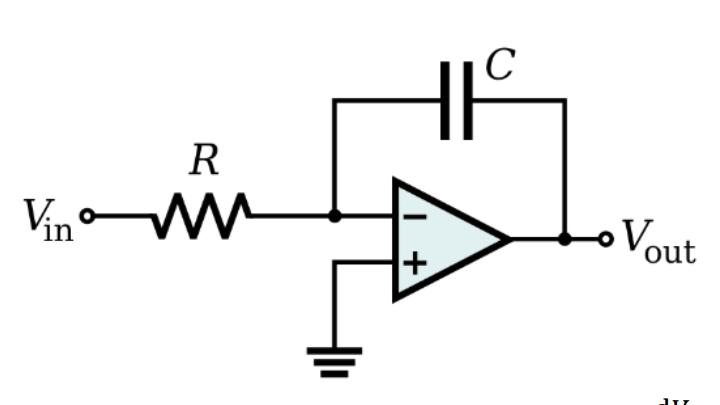
\includegraphics[width=0.5\textwidth]{integrator.png}
    \caption{An operational amplifier in an integrator setting}
    \label{fig:integrator}
\end{figure}
The input/output, or Transfer function, of the system can be written as follows:
\[
\frac{V_o}{V_i} = -\frac{z_2}{z_1} = \frac{-\frac{1}{Cs}}{R} = -\frac{1}{CRs}
\]
In this example, the capacitor \(C\) acts as an integrator, as it can be seen mathematically as \(H(s) = \frac{1}{s}\). In this case, if a unit step input is applied to the system, \(V_i(s) = \frac{1}{s}\), the output of the system is unbounded. It can be understood as follows:
\[
\lim_{t \to \infty} \int_{0}^{t} V_i(\tau) \, d\tau = 
\lim_{t \to \infty} \int_{0}^{t} \mathcal{E}(\tau) \, d\tau =
\lim_{t \to \infty} F(t) - F(0) = \lim_{t \to \infty} t - 0 = \infty
\]
which mean the system is BIBO unstable.
\end{example}
\begin{example}
Another example of integrator is a water reservoir.

Now, consider the following circuit, which is a resaunator circuit:

\begin{figure}[H]
    \centering
    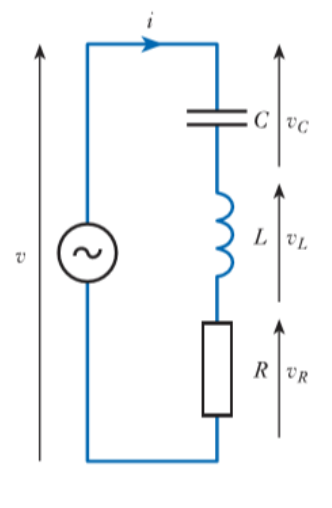
\includegraphics[width=0.25\textwidth]{resonator.png}
    \caption{a resonator circuit}
    \label{fig:resonator}
\end{figure}
The input-output relation of this circuit is as follows:
\[
I(s) = \frac{\frac{s}{L}}{s^2 + \frac{R}{L}s + \frac{1}{LC}} V(s)
\]
The natural frequency of this system is \(\omega = \frac{1}{\sqrt{LC}}\). If the value of the resistance \(R\) is zero in this system, by applying an input voltage with the aforementioned frequency, the current, theoretically, tends to infinity. 
\end{example}


In order for a system to be BIBO stable, the real part of all the poles of the system should be strictly smaller than zero.


\begin{QandAbox}[BIBO stable and Internally unstable]
Since there might be some cancellation between when shaping the transfer function of a system, \(H(s) = C(sI-A)^{-1}B + D)\), the poles of the system are a subset of the eigenvalues of the system matrix \(A\):\\

Poles(\(H(s)\)) \(\subseteq\) eig(\(A\)).\\

Hence, it can be concluded that if a system is asymptotically stable, then the system is also BIBO stable. However, the converse may not always be the case. Specifically, a system can be BIBO stable, but this does not guarantee that no zero-pole cancellation has occurred.\\

There may be cases where a system is \textbf{internally unstable} but \textbf{BIBO stable}. In such cases, one of the following two possibilities holds:

\end{QandAbox}
\begin{QandAbox}

\begin{itemize}
   \item The unstable mode of the system is \textbf{unreachable}, meaning that the input signal cannot stimulate that mode of the system.
   \item The unstable mode of the system is \textbf{unobservable}, meaning that while the input signal stimulates that mode, its effect does not appear in the output. This situation may lead to instability of the system itself.
\end{itemize}
\end{QandAbox}

The architecture of the control system discussed in this course is as follows:

\begin{figure}[H]
    \centering
    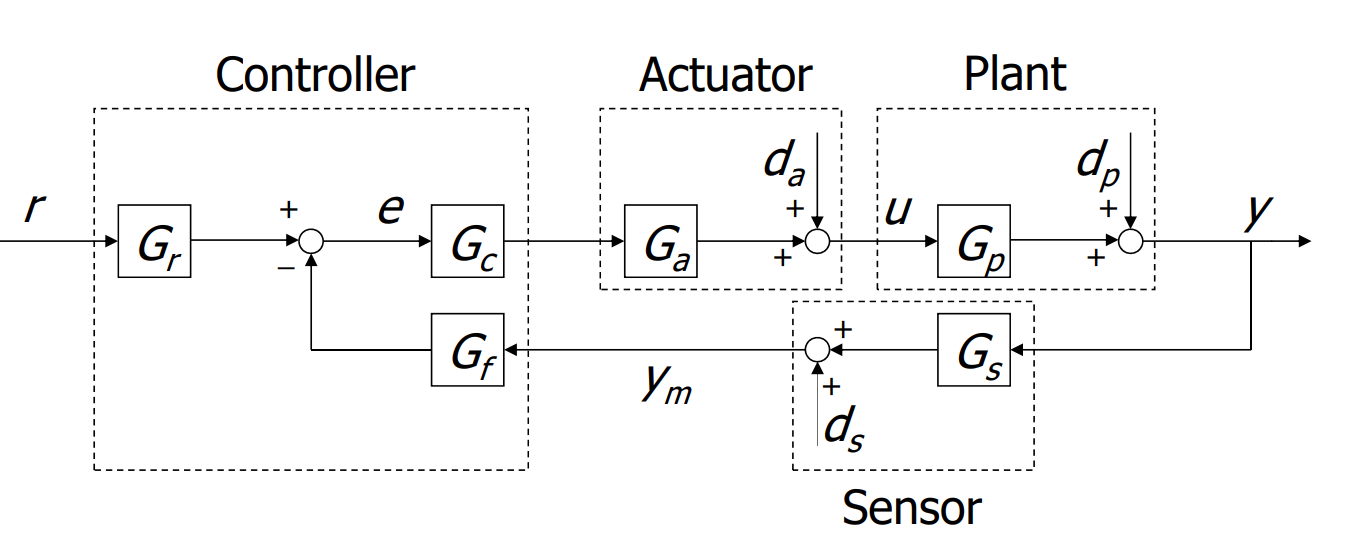
\includegraphics[width=0.75\textwidth]{control-architecture.png}
    \caption{The architecture of the control system discussed in this course}
    \label{fig:control-architecture}
\end{figure}
In the figure \ref{fig:control-architecture}, the symbols are as follows:
\begin{itemize}
    \item plant \(G_p\) with plant disturbance \(d_p\) 
    \item actuator \(G_a\) with actuator disturbance \(d_a\)
    \item sensor \(G_s\) with sensor noise \(d_s\)
    \item \textbf{cascade controller} \(G_c\)
    \item \textbf{feedback controller} \(G_f\), for 2 DoF or, if constant for dc-gain
    \item \textbf{prefilter} \(G_r\), also called reference generator
\end{itemize}

\textbf{Prefilter, or reference generator}, is not going to be discussed in this course. For instance, If an aircraft aims to land, the input of the system cannot be a step. The aircraft should follow a smooth path for landing. Therefore, prefilter does this job.

Let us consider the structure in the figure \ref{fig:our-control-system}. The multivariable transfer function \(M(s)\) from inputs signals \(r, d_u, \), and \(d_t\) to outputs signals \(e, u\), and \(y_m\) is given by:

\[
\begin{bmatrix}
e \\
u \\
y_m
\end{bmatrix}
=
\frac{1}{1 + PCF}
\begin{bmatrix}
1 & -PF & -F \\
C & 1 & -CF \\
PC & P & 1
\end{bmatrix}
\begin{bmatrix}
r \\
d_u \\
d_t
\end{bmatrix}
\]

\begin{figure}[H]
    \centering
    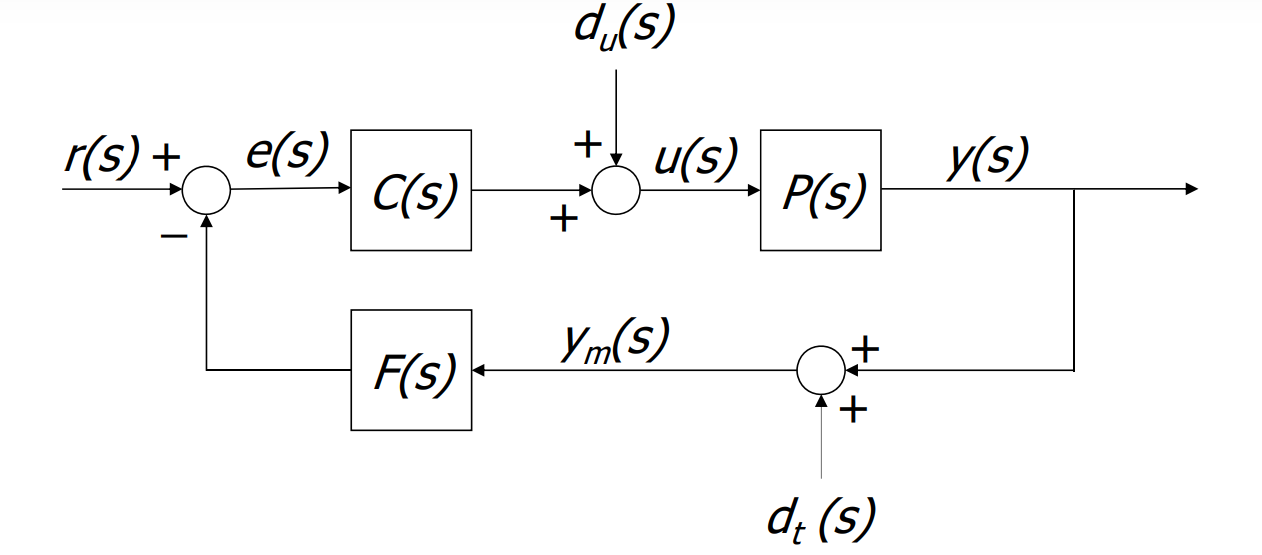
\includegraphics[width=0.75\textwidth]{our-control-system.png}
    \caption{The control architecture discussed for the following arguments}
    \label{fig:our-control-system}
\end{figure}

Based on this figure, we have the following definitions:
\begin{itemize}
    \item \textbf{loop-function} as\(L(s) = P(s)C(s)F(s)\)
    \item \textbf{sensitivity function} as \(S(s) =\left[1 + L(s)\right]^{-1}\)
    \item \textbf{complementary sensitivity function} as \(T(s) = 1- S(s)\)
\end{itemize}

\subsubsection{Well-posedness or closed-loop properness}
A feedback control system is said to be \textit{well-posed} or \textit{close-loop proper} if the closed-loop transfer function of every possible input-output pair of the system is proper.

The result of the \textit{well-posedness
}: The feedback control system is said to be well-posed if and only if:
\[
\lim \limits_{s \to \infty} \left\{1 + P(s)C(s)F(s)\right\} \neq 0
\]

\begin{factbox}[Physical interpretation of properness]
If the transfer fucntion of a physical system is not proper, in the time-domain, it implies that the state of the system at a given time instance depend on the future value of the input. This is in contradiction with causality, and therefore, physically unrealizable.

In the frequency domain, the final shape of the system's frequency response would be like that of a high-pass filter, meaning that the system would amplify high-frequency inputs, such as noise.
\end{factbox}

\subsubsection{Internal stability of feedback systems}
Let us assume that the plant \(P(s)\) to be controlled is \textit{\textbf{stabilizable}} by the input \(u\) - i.e. if all unstable modes are controllable - and \textit{\textbf{detactable}} through output \(y\) - i.e. if all unstable modes are observable. 

Having assumed that, the feedback system is said to be \textit{\textbf{internally stable}} if and only if the signals \(e, u\), and \(y_m\) are bounded for any possible choice of the bounded signals \(r, d_u\), and \(d_t\) - i.e if and only if all the transfer functions in \(M(s)\) are proper and BIBO stable.

\textbf{Results}:\\
The closed loop system considered here is stable if and only if the following considtions are met:
\begin{enumerate}
    \item all roots of the equation \(1 + L(s) = 0\) have real part strictly smaller than \(0\).
    \item there are no cancellations in \(\mathbb{Re}(s)\geq 0 \) when the product \(P(s)C(s)S(s)\) is formed.
\end{enumerate}

\textbf{Remarks}:
\begin{itemize}
    \item No proof is given.
    \item Consition (1) follows the fact that the poles of all the functions in \(M(s)\)) are roots of the equation \(1 + L(s) = 0\);
\end{itemize}


\chapter{Part2: Characteristics of SISO feedback control systems}

\section{Design objectives}
In the design of a feedback control system, the following objectives have to be taken into account.
\subsection{Internal stability of the feedback control system}
For all bounded distrubances and inputs, the system response at every point inside the controll loop must be bounded. The difference between internal stability and input-output stability was established in the previous part. \\
\begin{factbox}
It is possible for a system to be internally unstable and yet to have a stable stansfer function, i.e to be input-output stable. This happens when the system has unstable hidden modesl.
\end{factbox}

\subsection{Robust stability}
If the plant deviate from a nominal model, \textbf{a set of models} is suitable for a better erepresentation of the plant.\\
The set of models could be generated, for example, by letting the model parameters very over their uncertainty intervals, with each parameter value defining a member of teh set.\\
For a controller design to be acceptable, \textbf{the feedback control system must be internally stable for every model in the set.} This property is referred to as \textit{Robust stability}.
\subsection{Tracking}
A good feedback control system must provide satisfactory steady-state and transient tracking. It is not usually possible to have good tracking for all possible reference input. That is the reason why response specifications are normally given in the presence of specific reference signals or classes of signals.

\subsection{Disturbance attenuation/rejection}
It is common to examine in some detail the response to polynomial disturbances and sinusoidal disturbances.

\section{Relative stability}
In the design of a control system, it is required that the system be stable. Further, it is necessary that the system has adequate relative stability. Consider the following figures.
\begin{figure}[H]
    \centering
    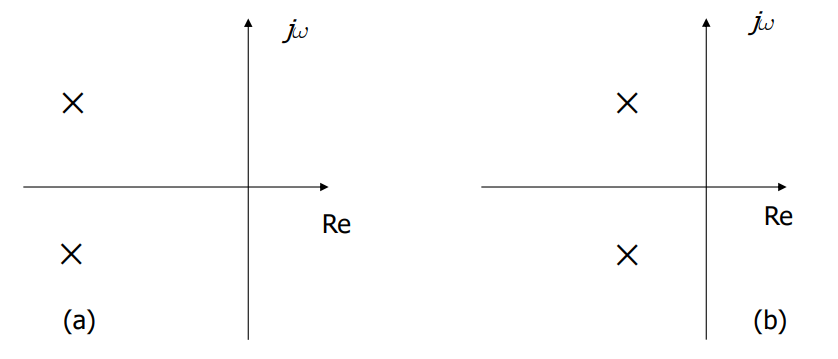
\includegraphics[width=0.75\textwidth]{relative-stability-01.png}
    \caption{The position of the poles of two system in \(S\)-plane; the system on the left represent a higher relative stability, since it is farther from the horizental axis, which is the verge of instability.}
    \label{fig:relative-stability-01}
\end{figure}

\begin{figure}[H]
    \centering
    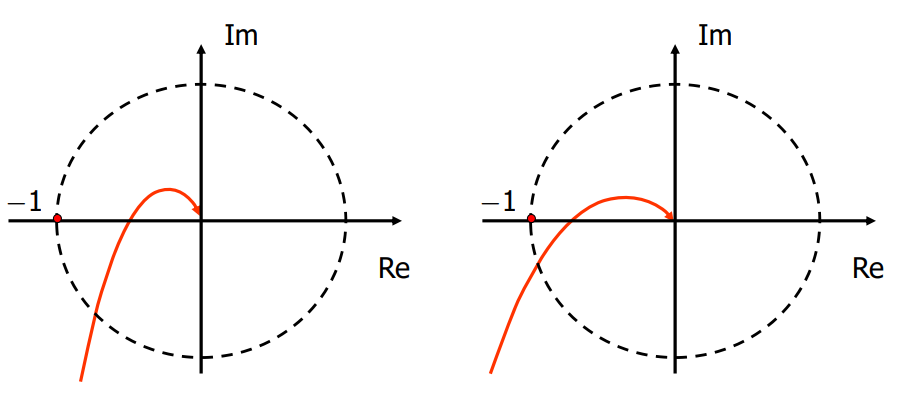
\includegraphics[width=0.75\textwidth]{relative-stability-02.png}
    \caption{The polar plot of the frequency response of two different systems; the system on the has a higher relative stability, since it has a large value of GM and PM.}
    \label{fig:relative-stability-02}
\end{figure}

In both figures, the system on represented on the
left is more stable than the system on the right. In the first figure, the system on the left is farther in the LHP, and in the second plot, the system on the left has a higher value of PM and GM.

The Nyquist criterion is defined in terms of the (-1, 0) point on the polar plot or the 0dB, -180° point on the Bode diagram or lag-magnitude-phase diagram. The proximity  of the \(GH(j\omega)\) locus to this stability pooint is a measure of relative stability. Consider the following transfer function and its polar diagram.
\[
G(s)H(s) = \frac{K}{s(\tau_1s +1)(\tau_2s+1)}
\]

\begin{figure}[H]
    \centering
    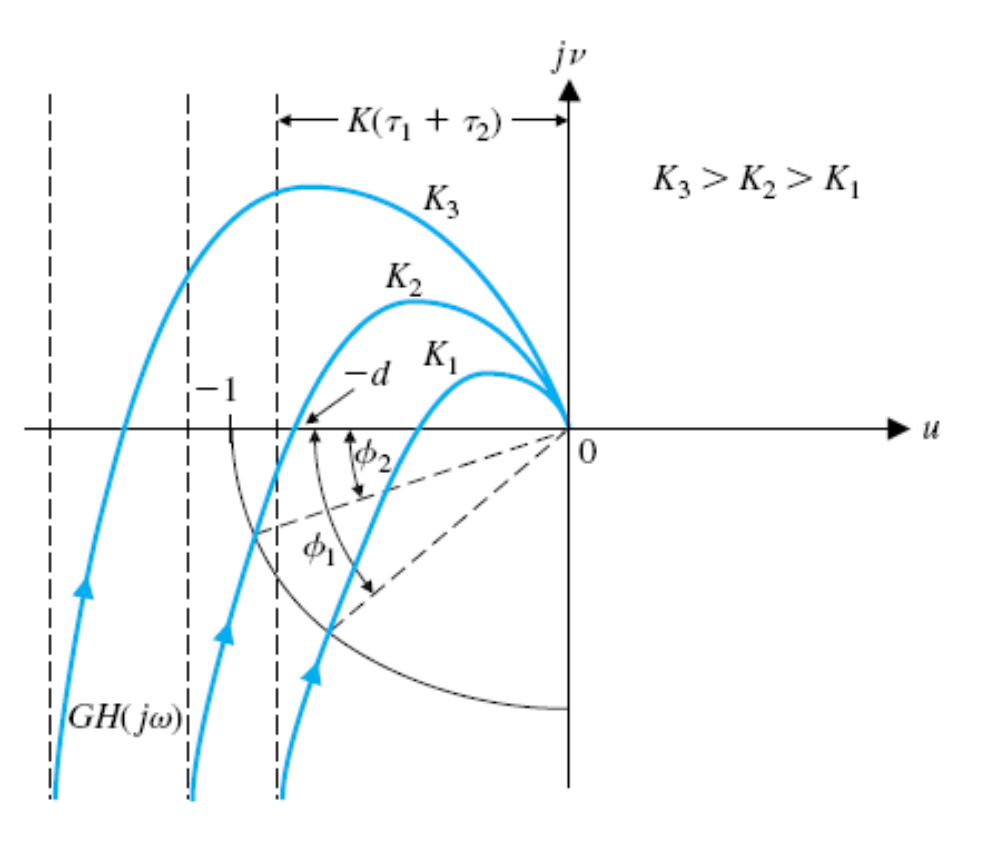
\includegraphics[width=0.5\textwidth]{relative-stability-03.png}
    \caption{The polar plot of the aforementioned transfer function for different value of gain \(K\).}
    \label{fig:relative-stability-03}
\end{figure}

FOR LOOP SHAPING LOOK AT THE NOTES MAKE FOR THE RESPONSE OF TEH LABS.

THIS PART CAN BE COMPLETED LATER IF IT IS NEEDED.

\chapter{Performance Specifications and Weighting Functions}

\section{Introduction}
In this part, the specifications are translated into constraints on sensitivity or complementary sensitivity functions. It is much more convenient to reflect given performance specifications by choosing suitable frequency dependent weighting functions.

Requirements can be written in a more compact way through the following constraint:
\[
W_s(j\omega)S(j\omega)) \leq 1 \: \forall \omega
\]
Where, $W_s(j\omega)$ is suitably chosen.

\begin{factbox}
In this part, both $G_a$ and $G_s$ are considered to be constant. This is due to the fact that \textbf{the bandwidth of actuator and sensor, must be much larger than the controller being designed.}; that is their dynamics are much faster than the dynamics of the system, and therefore, are neglected. If $G_f$ is not constant, a 2 DoF architecture is considred for the controller.
\end{factbox}

\begin{QandAbox}[Important]
The number of zeros of sensitivity function $S(j\omega)$ at 0 of the S-plane is equal the system type of the loop function. 
\begin{figure}[H]
    \centering
    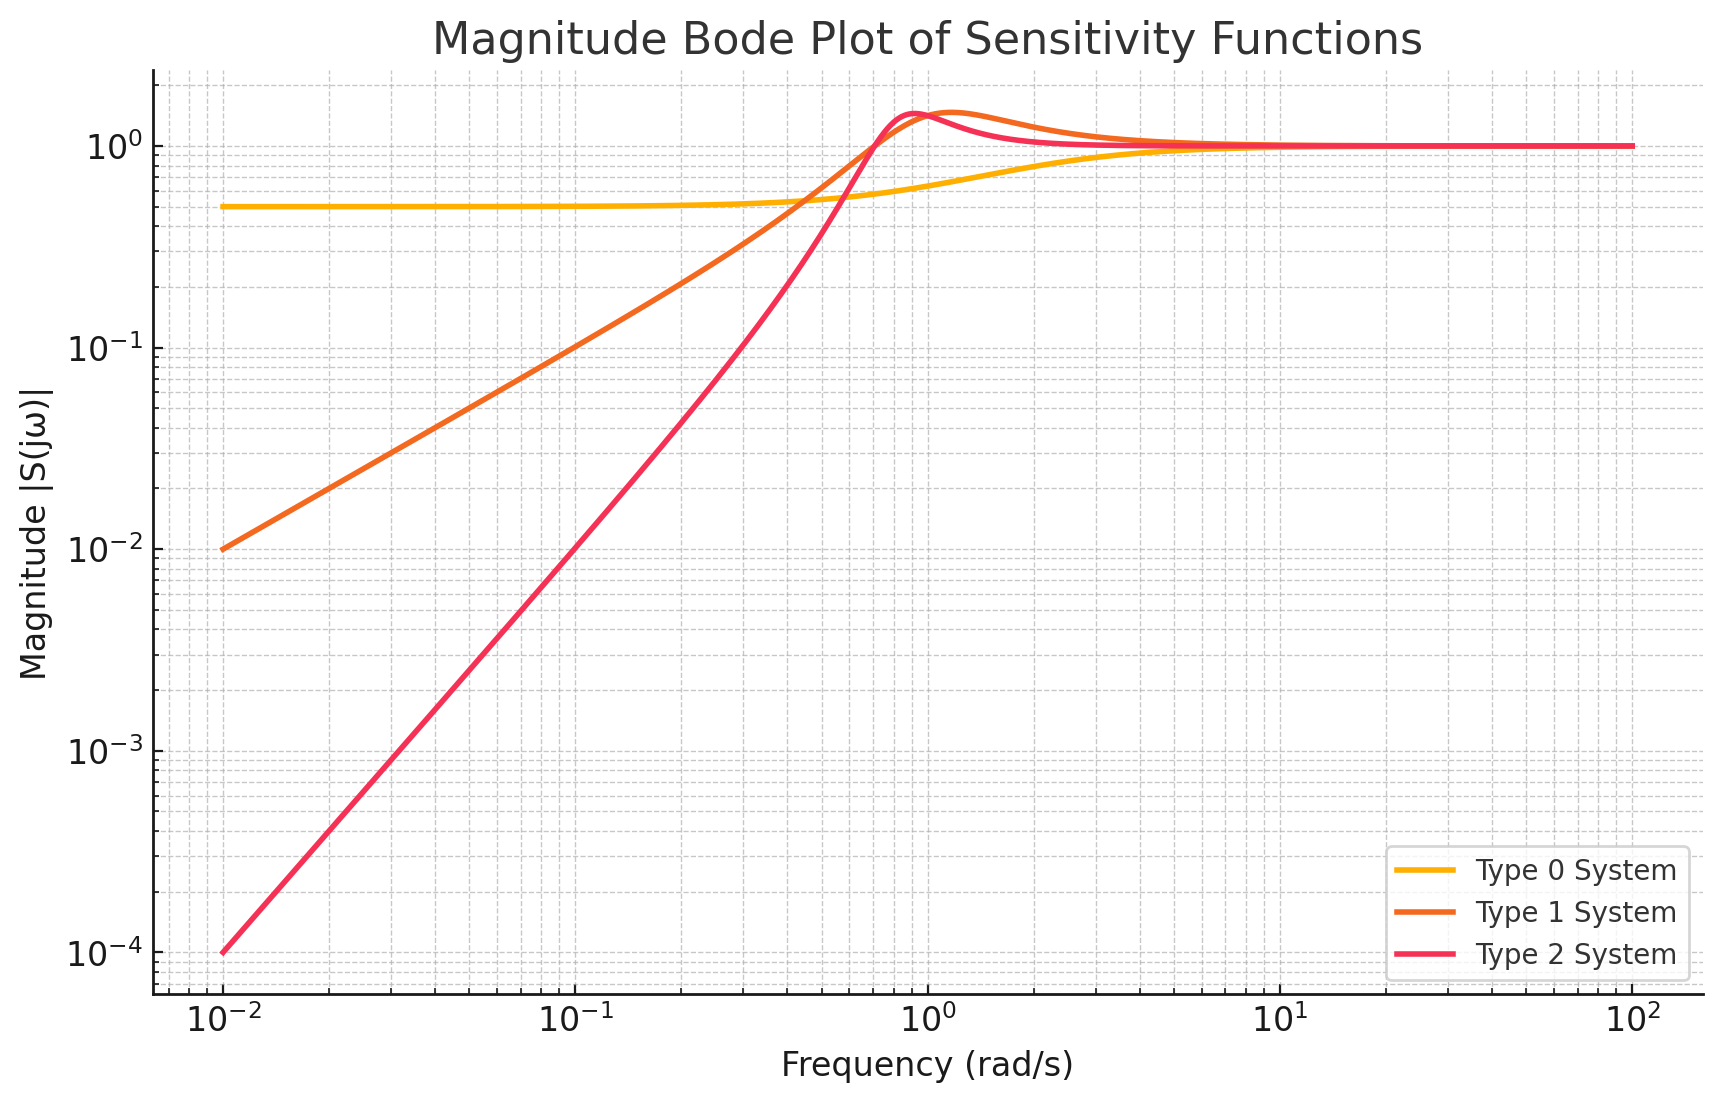
\includegraphics[width=0.75\textwidth]{sensitivity.png}
    \caption{The sensitivity function of 3 systems, the system type of which is indicated in the legend}
    \label{fig:sensitivity}
\end{figure}
One can realize that the sensitivity function of the second-order prototype has one zero at the origine, and therefore of system-type 1, but it is used for having a guidline studying transient requirements.
\[
S(s) = \frac{s(s+2\zeta\omega_n)}{s^2 + 2\zeta\omega_ns + \omega_n^2}
\]
\end{QandAbox}

A general sensitivity function $S(s)$, is considered as the follwoing form:\[
S(s) = s^{\nu + p}S^{*}(s)
\]
\newpage
\section{Steady-state resopnse to polynomial reference inputs}
For this class of specifications, the following form of constraint can be derived for $S^{*}(s)$.

\begin{figure}[H]
    \centering
    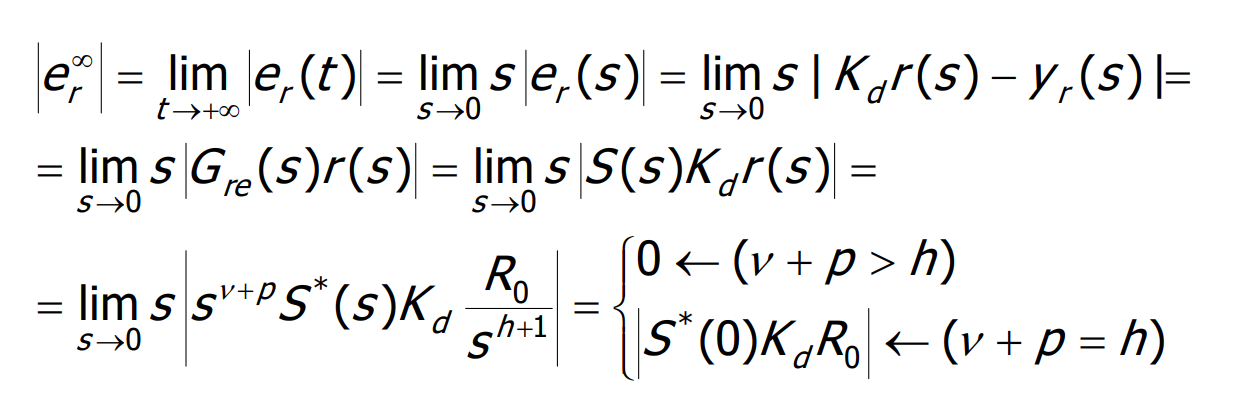
\includegraphics[width=0.5\textwidth]{ss-input.png}
    \caption{Constraint on the sensitivity function as a consequence of a specification on the steady-state input error at the presence of a polynomial input signal.}
    \label{fig:ss-input}
\end{figure}

In the case, $\rho_r = 0$ no constraint on the norm of $S^{*}$ is obtained. Also in the previous approach, if steady-state output error was required to be zero, no constriant on $K_c$ would be obtained.
\begin{factbox}[Some Reminders]
Having the frequency response of a function in the form of:
\[
H(s) = \frac{k_\nu}{s}\frac{(1 + \frac{s}{1})}{1 + \frac{s}{10}}
\]
the generalized dc-gain can be obtained in the following manner.
\begin{figure}[H]
    \centering
    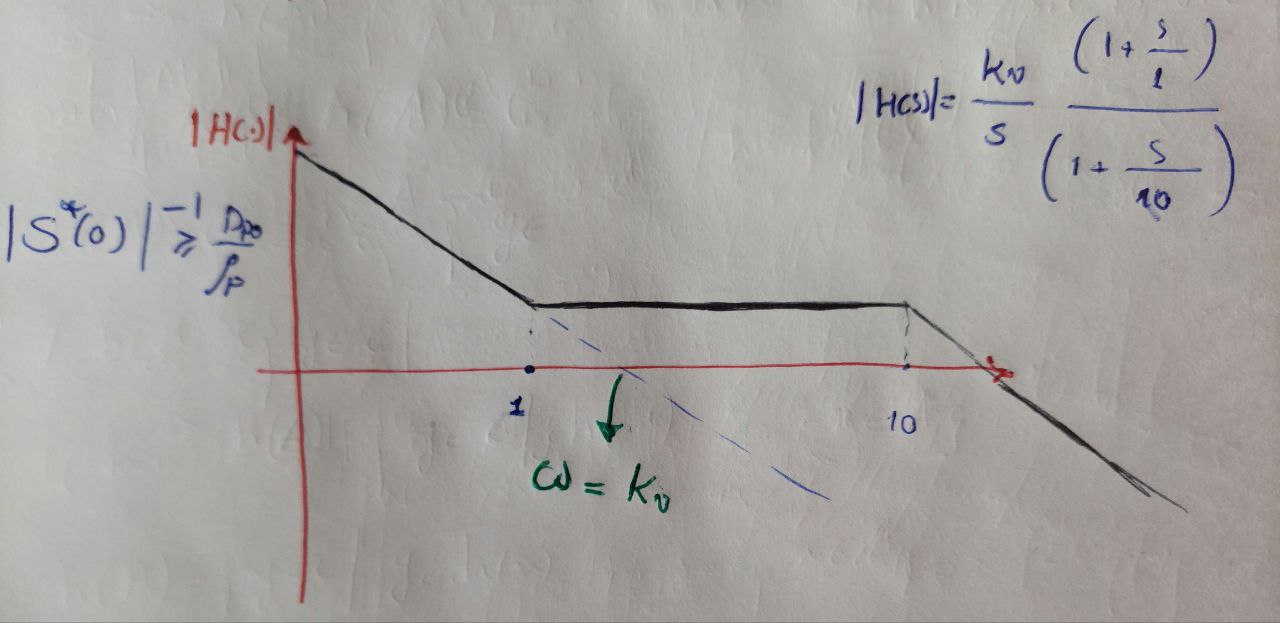
\includegraphics[width=0.75\textwidth]{dc-gain-s-1.jpg}
    \caption{}
    \label{fig:}
\end{figure}

Now, for the case that $H(s)$ has the same structure as sensitivity function.

\begin{figure}[H]
    \centering
    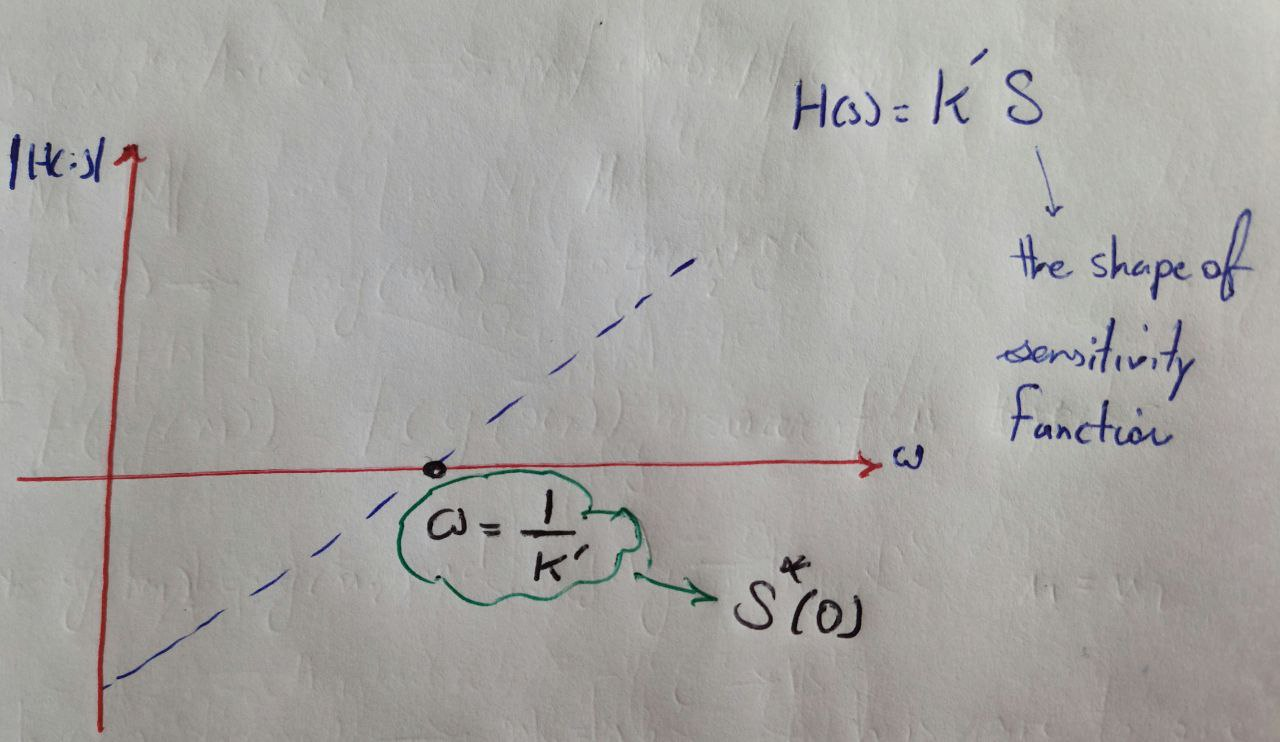
\includegraphics[width=0.75\textwidth]{dc-gain-s.jpg}
    \caption{}
    \label{fig:}
\end{figure}

\end{factbox}

\begin{factbox}[S-plane of the poles of a 2nd-order prototype system]
\begin{figure}[H]
    \centering
    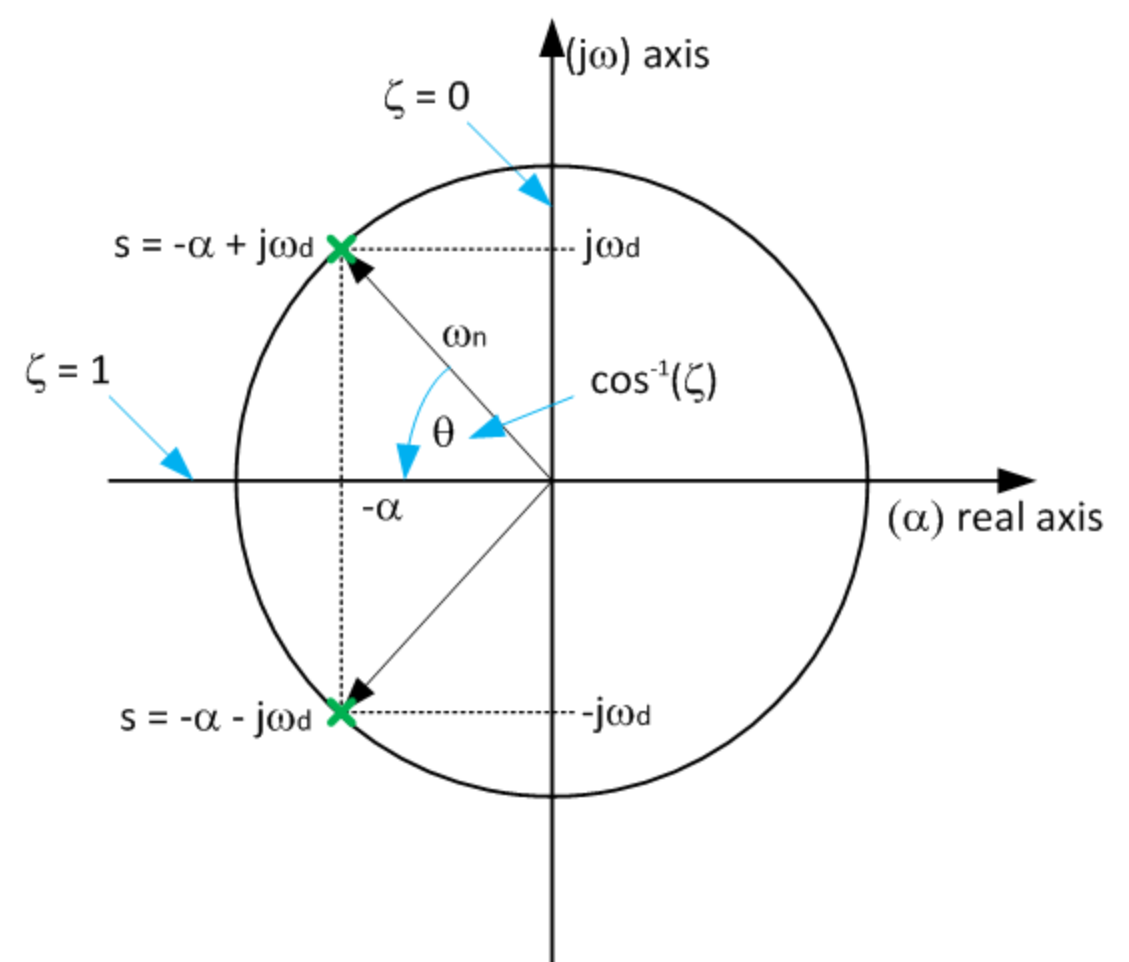
\includegraphics[width=0.5\textwidth]{s-plane.png}
    \caption{}
    \label{fig:}
\end{figure}
\end{factbox}

\section{Rational approximation of frequency constraints}
Rational functions of the variable $s$ are used to approximate the frequency domain constraints on $S$ and $T$. The parameters of the approximating fucntions(steady-state gain, zeros, and poles) can be moved to get the desired result. \textbf{Butterworth polynomials} can be used either as denominator or numerator of the approximating rational function to effectively retain constraints on different frequency ranges.

\subsection{Butterworth polynomials}

\begin{figure}[H]
    \centering
    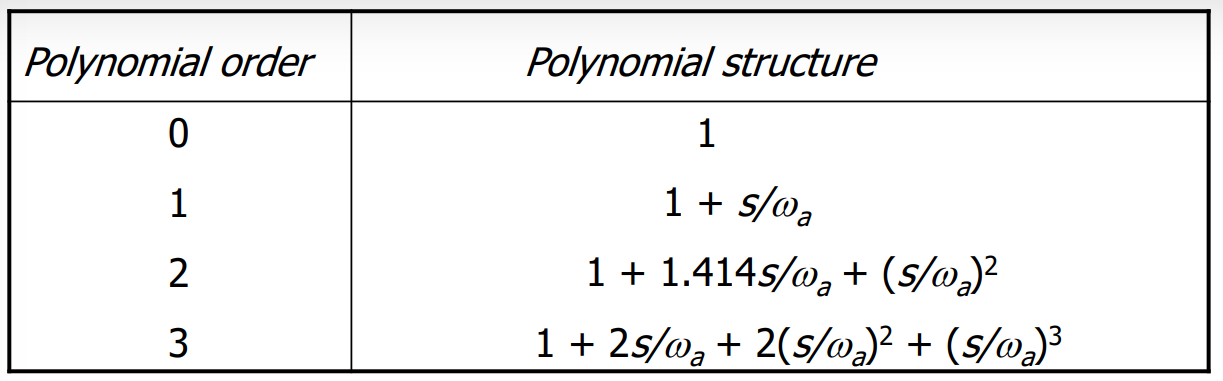
\includegraphics[width=0.75\textwidth]{butterworth.png}
    \caption{table of butterworth polynomials}
    \label{fig:butterworth}
\end{figure}

When a Butterworth polynomial is used as numerator (denominator) of a rational function, the magnitude of the frequency response at frequency $\omega_a$ is increased (decreased) by +3dB (-3dB) irrespective of the order of the polynomial.

Butterworth polynomials are used to obtain a rational function $W^{-1}_S(s)$ in such a way that $|W^{-1}_S(j\omega)|$ satisfies the constraints regarding $S(s)$.
\[
|W_S^{-1}| \leq M_S^{LF} \:\:\:\forall \omega_p \leq \omega_p⁺,\,\,\, \max\limits_{\omega}|W_S^{-1}(\infty)|\leq S_{p0}
\]
Butterworth polynomials are used to obtain a rational function $W_T^{-1}(s)$ in such a way that $|W^{-1}_T(j\omega)|$ satisfies:

\[
|W_T^{-1}| \leq M_T^{HF} \:\:\:\forall \omega_s \geq \omega_s^-,\,\,\, \max\limits_{\omega}|W_T^{-1}(\infty)|\geq T_{p0}
\]

$W_T^{-1}$ is required to satisfy:
\[
|W_T^{-1}| \leq M_S^{HF} \:\:\:\forall \omega_s \leq \omega_s⁻,\,\,\, |W_T^{-1}(0)|= T_{p0}
\]


\section{Performance specification as $H_{\infty}$ norm constraints}
Let us call:
\begin{itemize}
\item $W_S(s)$ the inverse of the rational approximation of the frequnecy domain constraints on the functiono $S(s)$
\item $W_T(s)$ the inverse of the rational approximation of the frequency domain constraints on the funtion $T(S)$
\end{itemize}

Design constraints obtained from the considered preformance requirements can be written in the following compact form:
\[
|T(j\omega)|\leq |W_T^{-1}|\,,\, |S(j\omega)| \leq |W_S^{-1}(j\omega)| \:\forall \omega
\]
or equivalently:
\[
|W_T(j\omega)T(j\omega) \leq \ \,,\, |W_S(j\omega)S(j\omega)|\leq \:\forall \omega
\]
Now, let us define the $H_{\infty}$ norm of a SISO LTI system with transfer function $H(s)$ as:
\[
\|H(s)\| := \max\limits_{\omega}|H(jw)|
\]
By exploring this definition, we can rewrite the design constraints obtained from the considered performance requirements in terms of the weighted $H_\infty$ norm of $S(s)$ and $T(s)$:
\[
\|W_T(s)T(s)\|_\infty \leq 1 \,,\, \|W_s(s)S(s)\|_\infty \leq \
\]

\begin{factbox}[information regarding the bode diagram of zeros and poles at 0]
example:
\(
H_1(s) = k_v \frac{H_1^*(s)}{s}
\),
here $v$ historically refer to velocity.
\end{factbox}

\section{Practicing shaping the weighting functions for sensitivity and complementary sensitivity function}
\begin{factbox}
Here, it is shown that how the frequency at which the asymptote of a transfer function passes the 0 dB axis is related to the DC gain of the transfer function.
\begin{figure}[H]
    \centering
    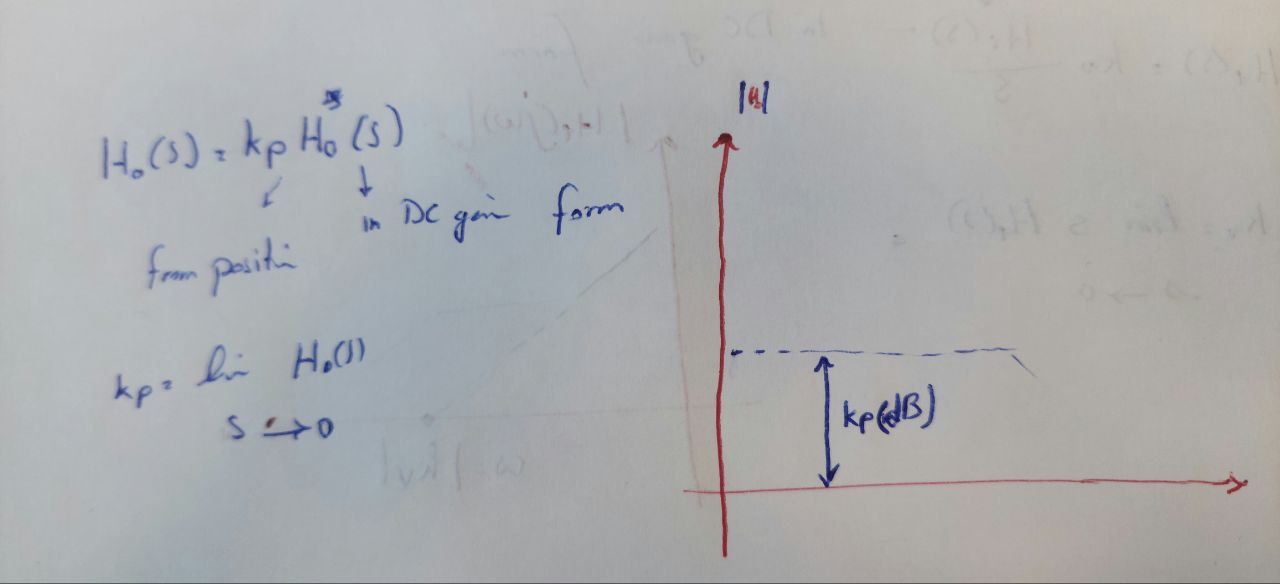
\includegraphics[width=0.75\textwidth]{H0.jpg}
    \caption{example 01}
\end{figure}
\begin{figure}[H]
    \centering
    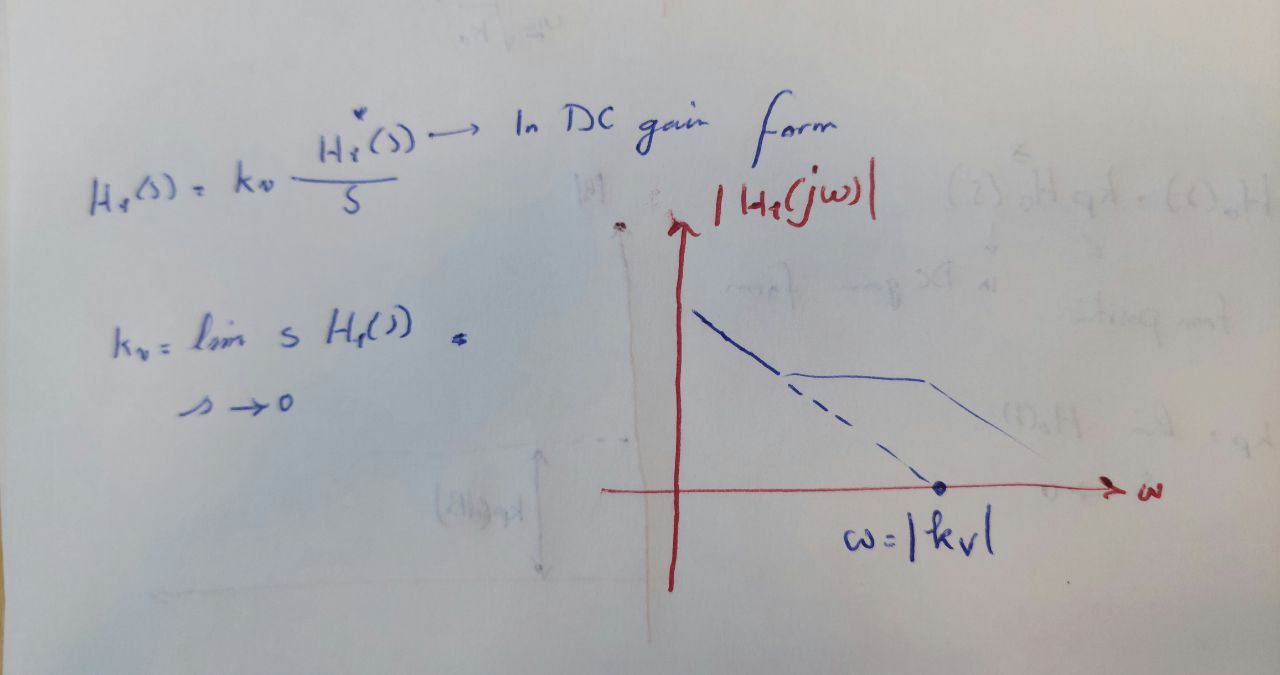
\includegraphics[width=0.75\textwidth]{H1.jpg}
    \caption{example 02}
\end{figure}
\end{factbox}

\begin{factbox}
\begin{figure}[H]
    \centering
    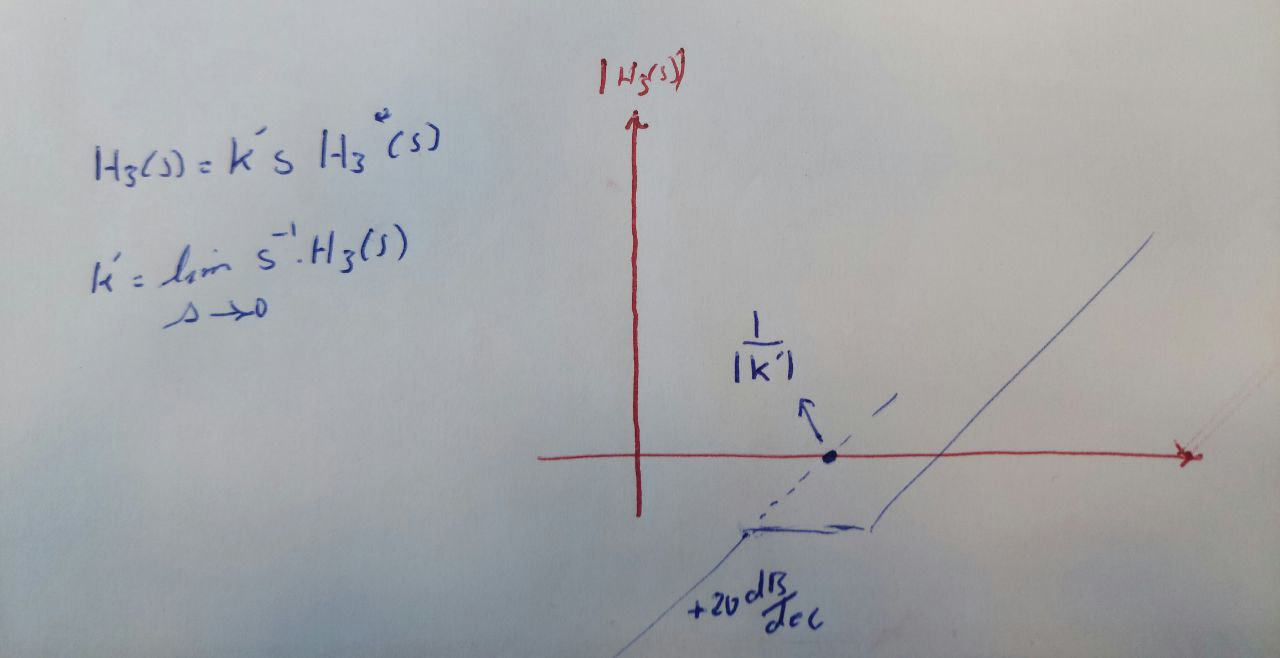
\includegraphics[width=0.75\textwidth]{H3.jpg}
    \caption{example 03}
\end{figure}
\begin{figure}[H]
    \centering
    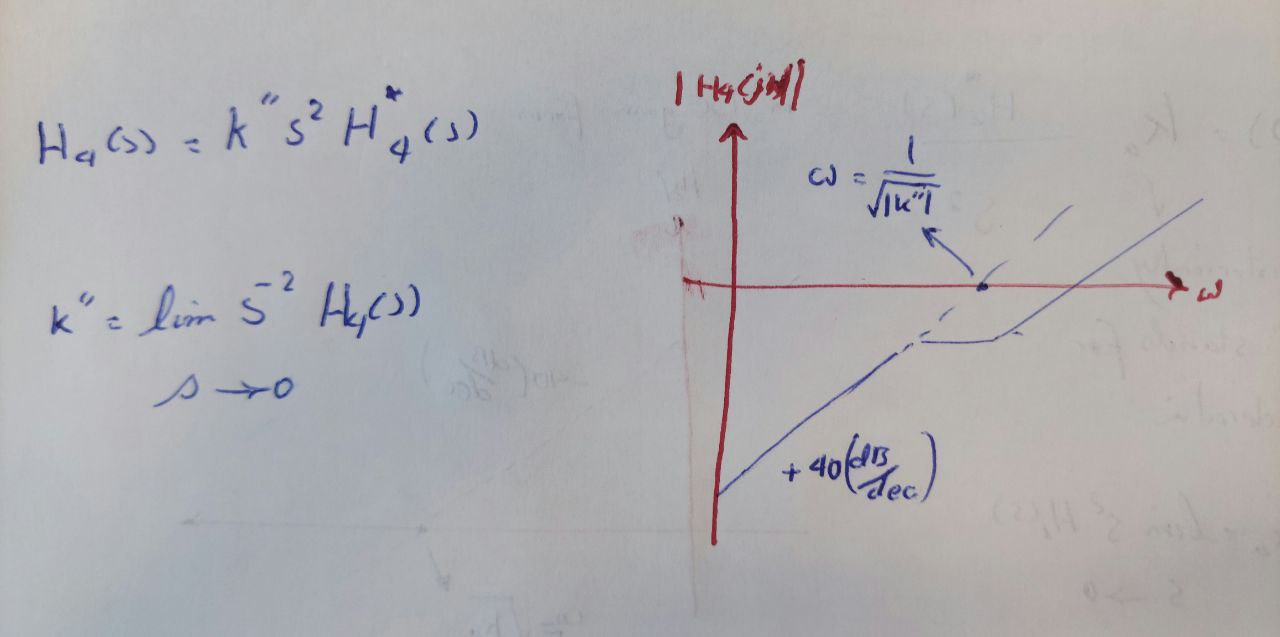
\includegraphics[width=0.75\textwidth]{H4.jpg}
    \caption{example 04}
\end{figure}
\end{factbox}

\section{shaiping the weight functions for S and T}
These weighting functions are going to be used in order to use the optimizer to obtain a controller in the $H_\infty$ method, as well as checking the robust stability and performance of the system final.


Just bear in mind that the weighting functions obtained in this stage are not exact, since we are using second-order prototype system for translating the requirements on the transient, and since we just use fractional transfer functions in order to shape the weight functions. \textbf{requirements on the steady-state performance are exact thanks to the fact that it depends on the known parameters like the system type of the system and disturbance assumptions.}

\subsection{Shaping $W_S$, the weighting function on the sensitivity funciton}
Consider the following constraints for our sensitivity function:
\[
M_S^{HF} = -60 \:dB \:\:\: \forall \:\omega \in (-\infty, \omega_p^{+}=1]
\]
\[
\zeta = 10 \:\% \: \Rightarrow \:\: S_{p_0} = 1.36
\]

The following weighting function can be considered as our first attempt:
\[
W_S^{-1} = k \frac{1 + \frac{s}{z_1}}{1 + \frac{s}{p_1}}
\]
where $ k = 0.001$ is equivalent to -60 $dB$. we put a zero at 1 in order to increase the magnitude, and \textbf{we compute the following limit in order to put our pole in a position to reach $S_{p0}$ when the frequency tends to infinity;} the reasult is a pole at $\omega = 1360 rad.sec^{-1}$.
\[
\lim\limits_{s \to \infty} W_S^{-1} = k \frac{p_1}{z_1} = S_{po} \Rightarrow p_1 = \frac{S_{p0}z_1}{k} = 1360
\]

\begin{figure}[H]
    \centering
    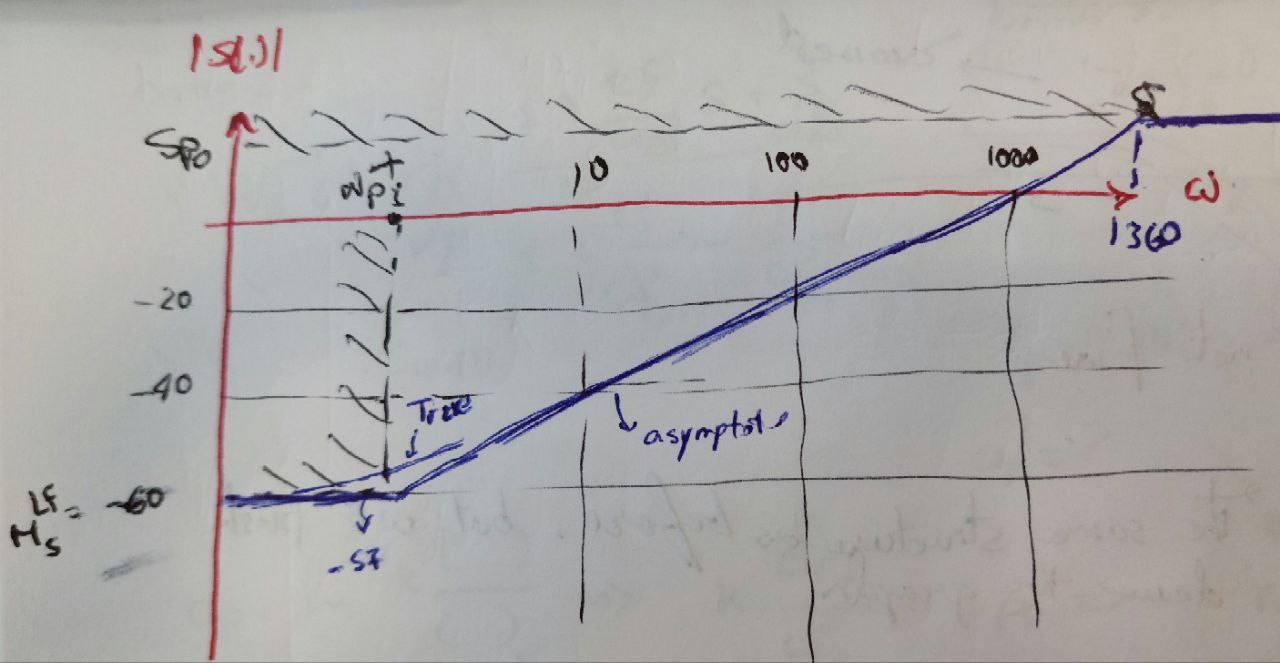
\includegraphics[width=0.75\textwidth]{ws-first.jpg}
    \caption{The first attempt to shape the weighting function}
\end{figure}

This solution is not fine, since based on the real behavior of the Bode of this transfer function, at $\omega = 1$, the magnitude increases by +3 $dB$, which is because of the first-order zero at $\omega = 1$, thereby passing the forbidden region; in other words, the requirement on the low frequency performance is not going to be satisfied. Another problem is that, having such a high crossover frequency and also taking into consideration the complementary sensitivity function, in this case $1000 Hz$, we may obtained infeasibility when optimizing for the controller.  \\

In the second attempt, one may decreases the value of dc-gain to $-63 dB$ in order to circumvent the first problem. However, doing so, the result of the limit which leads to the frequency of the pole leads to the frequency $1924$, making the situation even worst for the second issue.
\begin{figure}[H]
    \centering
    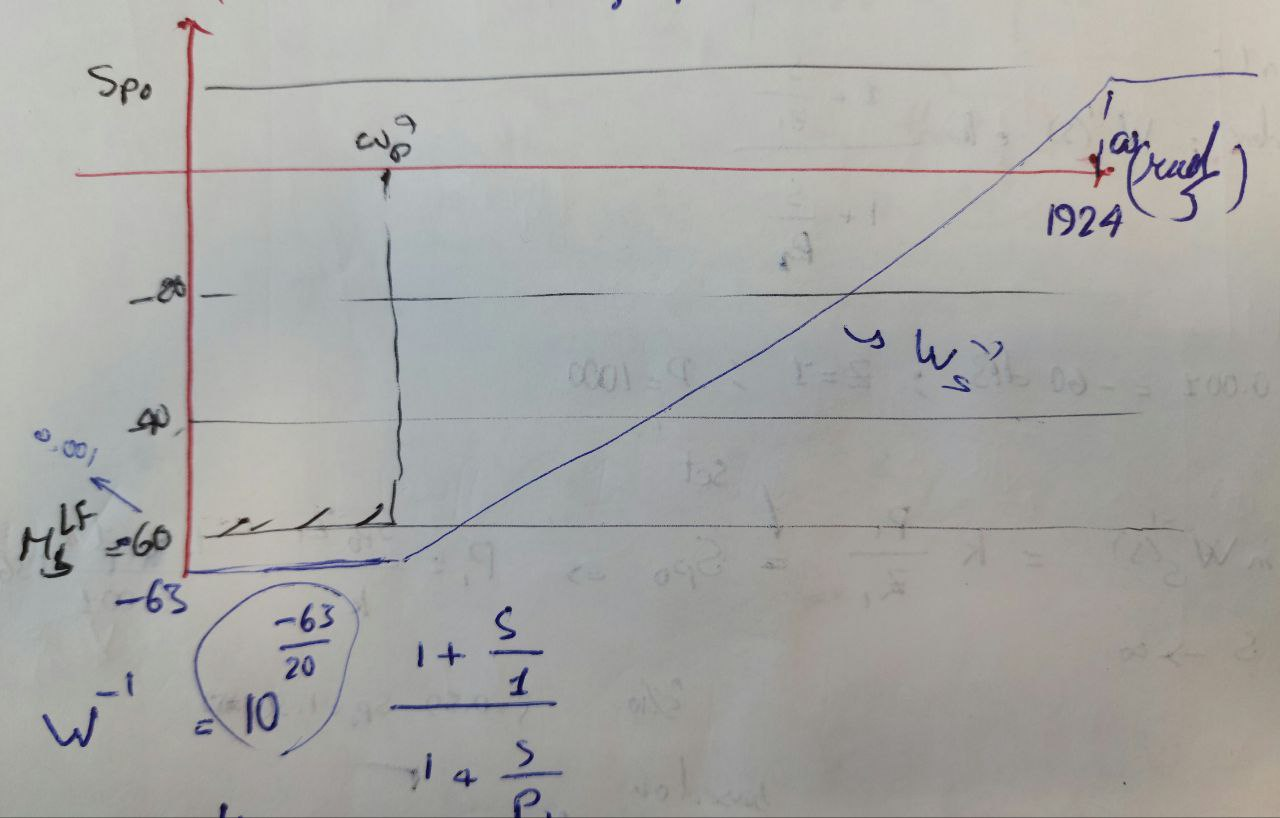
\includegraphics[width=0.75\textwidth]{ws-second.jpg}
    \caption{The second attempt to shape the weighting function}
\end{figure}


A third attempt might be using a butterworth polynomial in the both nominator and denominator of the weighting function. In this case, the both problems are tend to be solve, yet there is the chance that \textbf{the crossover frequency of $S$ become lower than requirements -  resulting in a slow transient performance due to the low crossover frequency.}\\

Considering the first problem of the homework, the system type of the loop function should be 1 so that the final system guarantees the steady-state performance requirements. \textbf{As the sensitivity function has the same number of zeros at 0 as the system type of the system.} so we start with the following inverse weighting function
\[
W_S^{-1} = s^{\nu + p} S^{*}(0) = 0.15s
\]
\textbf{consider that 0.15 determines some of the steady-state requirement performance for the sensitivity function, and the final dcgain of the sensitivity function should be less than this value. Leading to a higher $K_c$ in the loop shaping context.}

and then, we try to stay as close as possible to the prototype-second order system, due to the fact that the optimizer has a higher chance in order to find a solution that is as close as possible to a second order system. Finally, the limit should be used in order to make sure that when the frequency tends to infinity, the value of the inverse weighting function tends to $S_{p0}$. \\

The order of the zeros and poles to add to this first structure is as follows in the first attempt:
\begin{itemize}
    \item one zero to get close the second order prototype system.
    \item then, we need two poles in order to reduce the +40 slop to 0. when adding these poles, ideally we are willing to get as close as possible to the knee of the second-order sensitivity function.
\end{itemize}

The result is going to be like the follwoing figure.

\begin{figure}[H]
    \centering
    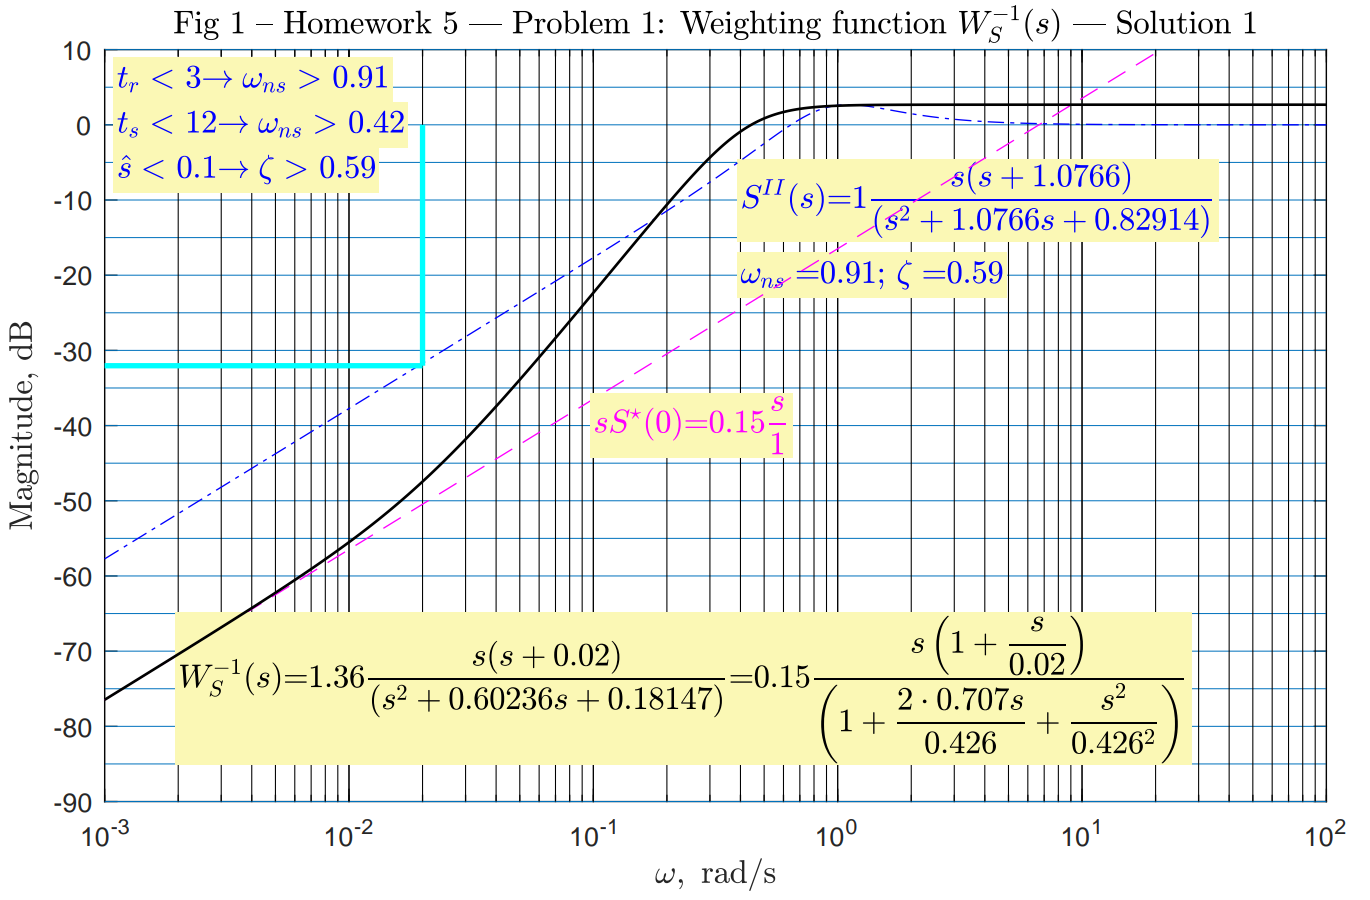
\includegraphics[width=0.75\textwidth]{h1-ws-first.png}
    \caption{The first attempt for $W_S^{-1}$ for the first problem of the homework.}
\end{figure}

As it can be seen, this weighting function may result in a slow system; As, in the contrary, if the crossover freequency is large than the one of thte second-order system, the resulting system is going to be faster than needed, or \textbf{bandwidth demanding}.

To resolve this issue, the position of the zero can be changed to a bit higher frequency in order to lead to the following result.

\begin{figure}[H]
    \centering
    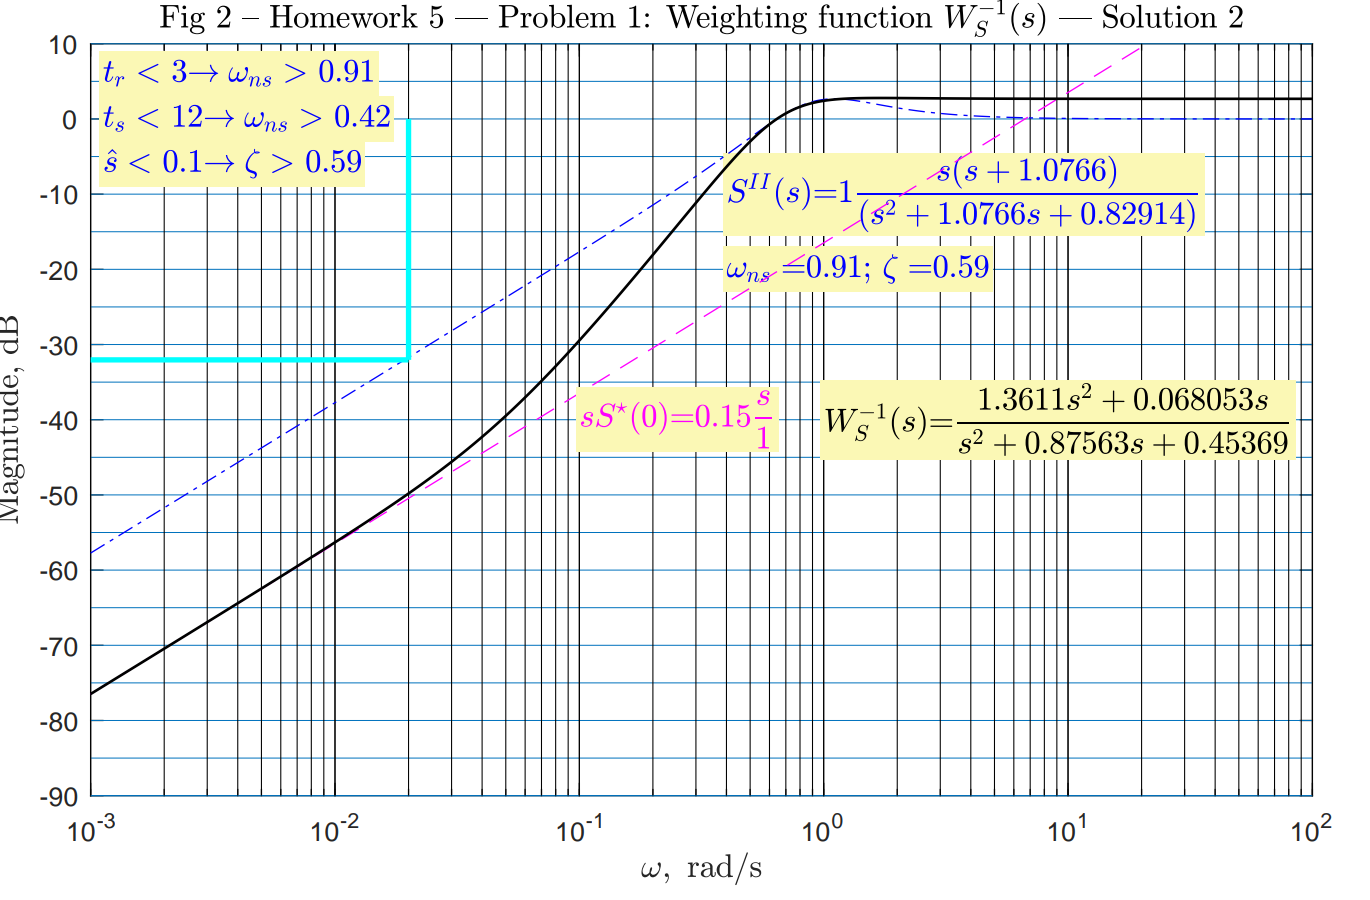
\includegraphics[width=0.75\textwidth]{h1-ws-second.png}
    \caption{The second attempt for $W_S^{-1}$ for the first problem of the homework.}
\end{figure}


To make the inverse weighting function to be tight as far as possible, the following weighting function can be used.

\begin{factbox}
According to the professor, the tightest the $W_S^{-1}$ to $S$, the simplest controller the optimizer is going to give.
\end{factbox}

A third attempt to make the weighting functino as tight as possible results in the following figure,

\begin{figure}[H]
    \centering
    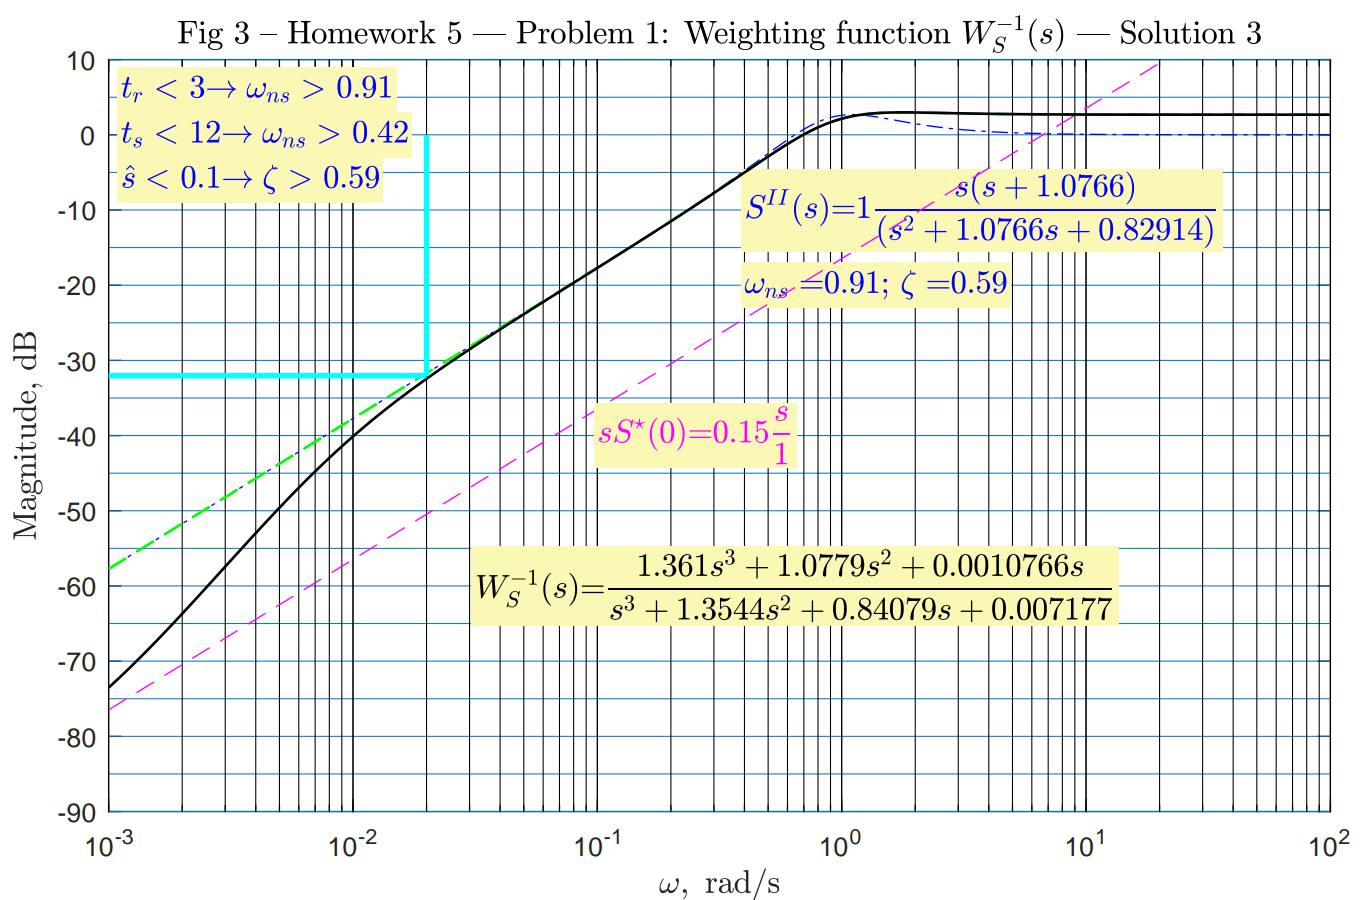
\includegraphics[width=0.75\textwidth]{h1-ws-third.png}
    \caption{The third attempt for $W_S^{-1}$ for the first problem of the homework.}
\end{figure}

In the end, $W_S$ is going to be simply the inverse of the $W_S^{-1}$

\subsection{Shaping $W_T$, the weighting function on the sensitivity funciton}
Here, it is much simpler. The procedure is as follows:
\begin{enumerate}
    \item We need to make sure that as $\omega$ tends to zero $W_T^{-1}$ is going to be at $T_{p0}$. Then, we start with
    \[
    W_T^{-1} = T_{p0}
    \]
    \item Then, we need to use a second-order butter worth function, and calculate the frequency of the poles so that the plot passes $M_T^{HF}$. The starting point is going to be as follows:
    \[
    T_{p0} - W_T^{-1}(\omega) = -40(\omega_p - \omega_s^{-})
    \]
    where
    $\omega_p$ is going to be used as the cutting frequency of the second-order butterworth function.
    
\end{enumerate}


\chapter{Unstructured uncertainty modeling and robustness}

\section{Unstructured uncertainty vs Structured uncertainty}
Regarding the physical aspect of uncertainty, irrespective of their complexity, mathematical models cannot exactly describe a real physical process. Sometimes, we may prefer simplified approximate models. Thus, model uncertainty has to be taken into account whne a mathematical model is used to analyze the behavior of a system to design a feedback control system.
\subsection{Source of model uncertainty}
The uncertainty in the mathematical models can stem from:
\begin{itemize}
    \item Intentional approximation of high-order or infinite-dimensional systems by low order models, e.g. neglected fast actuator and/or sensor dynamics.
    \item Neglected some or all high-frequency bending and torsional modes.
    \item Neglected far-away stable poles and/or far-away minimum and non-minimum phase zeros.
    \item Neglected small time delays (physical or computaitonal)
    \item Parameter uncertainty in coefficients of transefer functions 
    \item Neglected small non-linearities
\end{itemize}

\textbf{Model uncertainty is essentially due to:}
\begin{itemize}
    \item physical parameters not exactly known
    \item unmodeled (linear or nonlinear) dynamic
\end{itemize}

Uncertainty due to approximate knowledge of some parameter values is called \textbf{parameter uncertainty}\\
Uncertainty due to unmodeled dynamics is called \textbf{dynamic uncertainty}.\\

The basic approach to take uncertainty into account is to describe the plant under study as a member of a set of systems, also called \textbf{model set}. From now on, we will restrict our attention to LTI uncertain systems. Model sets for LTI uncertain systems can be classified as:
\begin{itemize}
    \item \textbf{Structured uncertainty model set}: when the set is parametrized by a finite number of parameters
    \item \textbf{Unstructured uncertainty model set}: when complete ignorance regarding the order and the phase behavior of the system is assumed.
\end{itemize}

\textbf{Parametric uncertainty} leads straightforwardly to \textbf{structured model sets}. It can also be described (with "some conservativeness") by means of \textbf{unstructured model sets.} \textbf{Dynamic uncertainty} leads straightforwardly to \textbf{unstructured model sets}.\\

Four different unstructured model sets will be considered, which will refer to:
\begin{itemize}
    \item additive uncertainty
    \item multiplicative uncertainty
    \item inverse additive uncertainty
    \item inverse multiplicative uncertainty
\end{itemize}
\begin{example}
In order to have an intuition about the set of models consider the following simple case:
\[
\alpha: 4\div8, \alpha \in \mathbb{R}
\]
Considering $\alpha_n$ as the nominal value of the parameter, we can consider the set of model $M$ as follow:
\[
M = \{\alpha: \alpha = \alpha_n + r\delta: \:\:\:\:\: |\delta| \leq 1; \: r = 2;\: \alpha = 6\}
\]
Here, the variable $r$ signifies the magnitude of the uncertainty. The larger $r$, the larger the uncertainty regarding the value of the parameter.
\end{example}

All in all, in order to model uncertainty in an unstructured manner, we should choose a nominal plant, and a weighting function $W_u$ quantifying the magnitude of uncertainty.

\subsection{The additive uncertainty model set}
The mathematical set of this kind of uncertainty model is as follows:
\[
M_a = \{G_p(s):\:G_p(s)\,=\,G_{pn}+W_u(s)\Delta(s),\,\|\Delta(s)\|_\infty\leq 1 \}
\]
where:$G_{pn}$ is the nominal model of the plant. $\Delta(s)$ can be any possible transfer function whose $H_\infty$ norm is less than 1. \textbf{$W_u(s)$ is weighting function which accounts for the size of the uncertainty}. 
\begin{QandAbox}
It is assumed that all systems belonging to $M_a$ must have the same number of unstable poles. 
\end{QandAbox}

\begin{figure}[H]
    \centering
    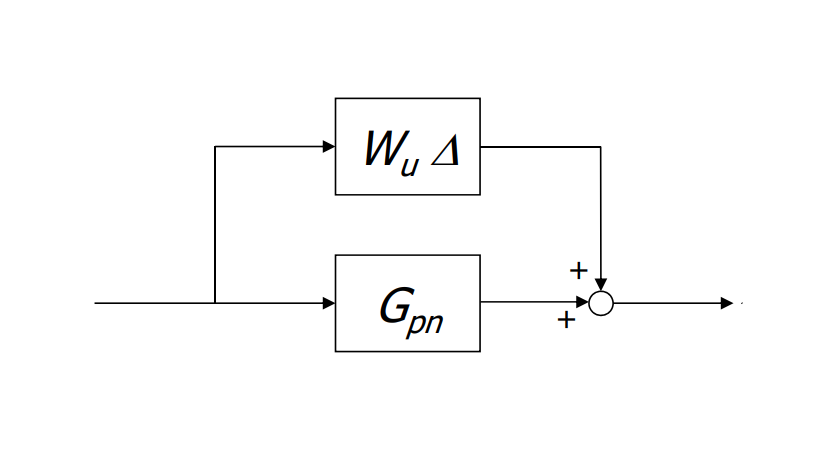
\includegraphics[width=0.5\textwidth]{additive-uncertainty.png}
    \caption{The block diagram description of additive uncertainties}
    \label{fig:sensitivity}
\end{figure}

\subsubsection{Use cases:}
\begin{enumerate}
    \item \textbf{Disturbances and External Noise Influences:}\\
    \textbf{Scenario:} When the system experiences external disturbances that add to its output directly (e.g., sensor noise, external forces, or environmental disturbances).\\
\textbf{Why Additive:} The uncertainty does not affect the system's internal dynamics but introduces variation at the output.\\
\textbf{Example:} A temperature sensor in a heating system where fluctuations in room temperature due to external drafts or minor noise in measurement affect the output but not the heater’s internal dynamics.
    \item \textbf{Low-Frequency Uncertainty Dominance:}\\
    \textbf{Scenario:} When uncertainty is mainly present at low frequencies, where it can dominate system behavior.\\
\textbf{Why Additive:} At low frequencies, the additive model is effective as it can capture steady-state or slow-moving disturbances, which are common in control applications.\\
\textbf{Example:} An aircraft with control surfaces that may experience slow, random wind gusts affecting the output position without impacting the fundamental control dynamics.
    \item \textbf{Unmodeled Dynamics Outside the Bandwidth of Interest:}\\
  \textbf{Scenario:} When there are unmodeled high-frequency dynamics that don’t impact the primary system response but could affect output measurements.\\
\textbf{Why Additive:} Additive uncertainty is often used to approximate unmodeled dynamics that are outside the control bandwidth but might still show up in system outputs.\\
\textbf{Example:} A robotic arm with minor high-frequency oscillations in its joints; while these oscillations are outside the primary control bandwidth, they are added as uncertainties in the output.
    \item \textbf{Unmodeled Dynamics Outside the Bandwidth of Interest:}\\
    \textbf{Scenario:} When there are unmodeled high-frequency dynamics that don’t impact the primary system response but could affect output measurements.\\
\textbf{Why Additive:} Additive uncertainty is often used to approximate unmodeled dynamics that are outside the control bandwidth but might still show up in system outputs.\\
\textbf{Example:} A robotic arm with minor high-frequency oscillations in its joints; while these oscillations are outside the primary control bandwidth, they are added as uncertainties in the output.
    \item \textbf{Measurement Uncertainties at System Output:}\\
   \textbf{ Scenario:} When the primary source of uncertainty arises from inaccuracies in measurement rather than the system's internal dynamics.\\
\textbf{Why Additive:} Measurement noise or sensor errors can often be well-represented by additive uncertainty since they appear at the output stage.\\
\textbf{Example:} In a feedback control system for temperature regulation, if the thermocouple sensor has random noise, this noise can be treated as an additive uncertainty.
\end{enumerate}

\begin{example}
consider a plant described by the following transfer function:
\[
G_p(s) = \frac{1}{\left( \frac{s}{5} + 1 \right) \left( \frac{s^2}{2500} + \frac{s}{2500} + 1 \right) \left( \frac{s^2}{6400} + \frac{1.6s}{6400} + 1 \right)}
\]
This is the transfer function of an electrical motor. The slowest pole correspond to the mechanical dynamic of the system. The other two poles which are faster, correspond to the electrical poles. Assume that in order to simplify the plant model to be used in controller design, we neglect the flexible modes. This is equivalent to chose thet following transfer function for nominal model:
\[
G_{pn}(s)=\frac{1}{(1+\frac{s}{5})}
\]
\textbf{In order ot descirbe the uncertainty due to the unmodelled dynamics which corresponds to the flexible modes, we considder and additive uncertainty model set.}
$G_p$ has one real pole and two pairs of lightly damped complex-conjugate poles (flexible modes). \\
Assume that in order to simplify the plant model to be used in the controller design, we neglect the flexible modes. This is equivalent to choose the following transfer function for the nominal model:\\
\[
G_{pn} = \frac{1}{\frac{s}{5}+1}
\]
\end{example}
In order to describe the uncertainty due to the unmodeled dynamics which corresponds to the flexible modes, we consider an additive uncertainty model set.
The following additive uncertainty model set is considered 
\[
M_a = \{G_p(s): G_p(s) = G_{pn} + W_u(s)\Delta(s), \|\Delta(s)\|\leq 1\}
\]
where, by construction, the weighting function $W_u$ must satisfy the following condition:
\[
\|\frac{G_p(s)-G_{pn}(s)}{W_u(s)}\|_\infty = \|\Delta(s)\|_\infty \leq 1
\]
which is equivalent to:
\[
|G_p(j\omega)-G_{pn}(j\omega)| \leq |W_u(j\omega)| \:\:\forall \omega
\]


\begin{figure}[H]
    \centering
    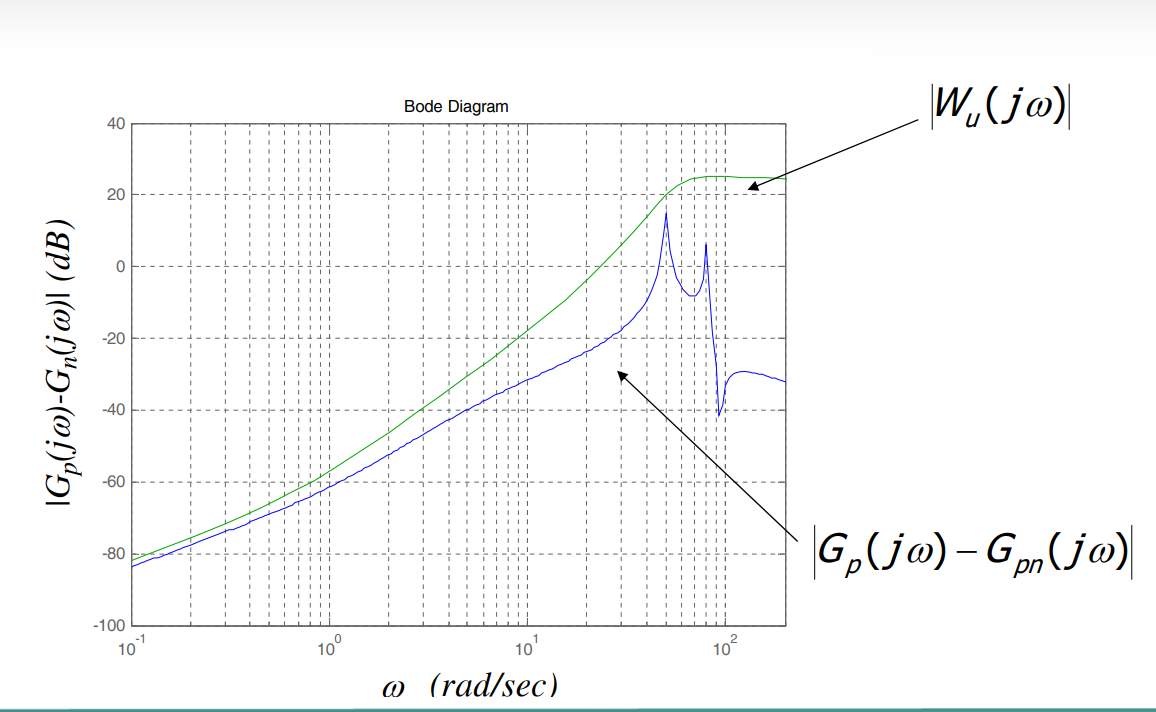
\includegraphics[width=0.75\textwidth]{additive-weighting.png}
    \caption{A possible weighting function describing the unstructured uncertainty that is modelled in an additive manner.}
\end{figure}

Pay attnetion that this weighting function should be as tight as possible in order to reduce the conservativeness.


\subsection{The multiplicative uncertainty model set}
The mathematical set of this kind of uncertainty model is as follows:
\[
M_m = \{G_p(s):\:G_p(s)\,=\,G_{pn}[1 + W_u(s)\Delta(s)],\,\|\Delta(s)\|_\infty\leq 1 \}
\]
where:$G_{pn}$ is the nominal model of the plant. $\Delta(s)$ can be any possible transfer function whose $H_\infty$ norm is less than 1. \textbf{$W_u(s)$ is weighting function which accounts for the size of the uncertainty}. 
\begin{QandAbox}
??It is assumed that all systems belonging to $M_m$ must have the same number of unstable poles. ?? Not written in the slides
\end{QandAbox}

\begin{figure}[H]
    \centering
    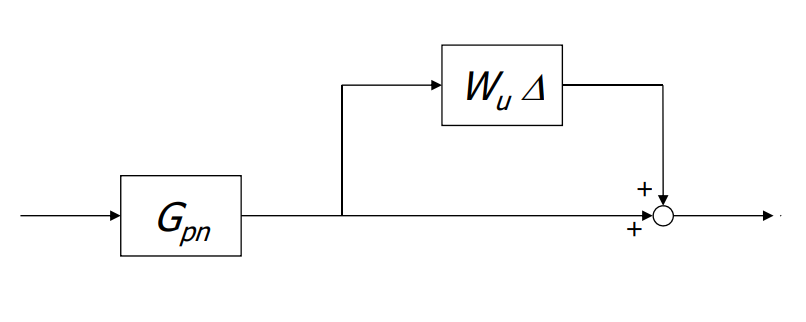
\includegraphics[width=0.5\textwidth]{multiplicative-uncertainty.png}
    \caption{The block diagram description of multiplicative uncertainty}
\end{figure}
Considering the formulation of the problem, the weighting function $W_u$ must satisfy the following condition:
\[
\|(\frac{G_p(s)}{G_{pn}}-1)\frac{1}{W_u(s))}\|_\infty = \|\Delta(s)\|_\infty \leq 1
\]
which is equivalent to:
\[
|(\frac{G_p(s)}{G_{pn}}-1)| \leq |W_u(j\omega)| \:\: \forall \omega
\]
here, $G_p$ represents the whole family.
\subsubsection{Use cases:}
\begin{enumerate}
    \item \textbf{Modeling Uncertainties in Plant Dynamics:}\\
    \textbf{Scenario:} When uncertainties arise directly in the plant's dynamics, affecting the system’s behavior multiplicatively (e.g., gain or phase variations).\\
    \textbf{Why Multiplicative:} The uncertainty scales with the nominal system dynamics, making multiplicative uncertainty ideal for capturing such variations.\\
    \textbf{Example:} In an electronic circuit, variations in component values (e.g., resistance, inductance) lead to changes in the system gain or frequency response, which are proportional to the nominal dynamics.

    \item \textbf{High-Frequency Uncertainty Dominance:}\\
    \textbf{Scenario:} When the system’s response at high frequencies is uncertain due to unmodeled dynamics or parameter variations.\\
    \textbf{Why Multiplicative:} At high frequencies, uncertainties often scale with the system's dynamics, as unmodeled dynamics or delays tend to affect system performance multiplicatively.\\
    \textbf{Example:} An aircraft experiencing structural flexibilities at high frequencies where these unmodeled dynamics alter the transfer function of the nominal model.

    \item \textbf{Frequency-Dependent Plant Gain Variations:}\\
    \textbf{Scenario:} When the gain or phase of the system varies with operating conditions or frequency.\\
    \textbf{Why Multiplicative:} Gain variations at specific frequencies are well-captured by scaling the nominal plant model by an uncertainty term.\\
    \textbf{Example:} A motor whose torque output depends on frequency, where small deviations in frequency lead to proportional changes in output gain.

    \item \textbf{Unmodeled Dynamics Near Control Bandwidth:}\\
    \textbf{Scenario:} When the primary concern is unmodeled dynamics near or within the system’s control bandwidth.\\
    \textbf{Why Multiplicative:} Unmodeled dynamics close to the system's natural frequency often affect the plant’s behavior in a manner proportional to its nominal transfer function.\\
    \textbf{Example:} A robotic arm where flexible joint dynamics close to the control bandwidth lead to uncertain oscillatory behaviors.

    \item \textbf{Process Variations in Gain or Time Delay:}\\
    \textbf{Scenario:} When physical parameters like gain or time delay are subject to process variations due to manufacturing tolerances or operational conditions.\\
    \textbf{Why Multiplicative:} Variations in these parameters influence the plant transfer function multiplicatively, altering both the magnitude and phase of the response.\\
    \textbf{Example:} A chemical reactor where temperature-dependent reactions cause the plant's time constants to vary proportionally with operating conditions.
\end{enumerate}

\begin{example}
Consider a plant described by the following transfer function
\[
G_p(s) = \frac{K}{s-2}
\]
where $K$ is an uncertain real constant which satisfies:
\[
5 \leq K \leq 15
\]
Here, it is shown that \textbf{the parametric uncertainty can be described by means of a multiplicative uncertainty model set}.
\[
M_m = \{G_p(s):\:G_p(s)\,=\,G_{pn}[1 + W_u(s)]\Delta(s),\,\|\Delta(s)\|_\infty\leq 1 \}
\]
The problem is to properly \textbf{select the nominal model $G_{pn}$ in order to minimize the size of unstructured uncertainty $W_u$} used to describe the parametric uncertainty.\\
Let's consider the following structure for the nominal model:
\[
G_{pn}(s)=\frac{K_n}{s-2}
\]
where $K_n$ is a constant value to be computed.

\end{example}

The weighting function $W_u$ must satisfy the following condition:
\[
\|\Delta(s)\|_\infty = \sup\limits_{\omega} \left| \left( \frac{G_p(j\omega)}{G_{pn}(j\omega)} - 1 \right)\frac{1}{W_u(j\omega)} \right| \leq 1
\]
which is equivalent to:
\[
|W_u(j\omega)| \geq \left| \frac{G_p(j\omega)}{G_{pn}(j\omega)} - 1 \right| \geq \left| \frac{K}{K_n} - 1 \right| \:\: \forall \omega , \, \forall K
\]
$K_n$ can be selected in order to minimize the size of the uncertainty, that is,
\[
|W_u(j\omega)| \geq \min\limits_{K_n} \max\limits_{K} \left| \frac{K}{K_n} - 1 \right| \:\:\:\:\: \forall \omega
\]
It can easily be shown that:
\[
\min\limits_{K_n} \max\limits_{K} \left| \frac{K}{K_n} - 1 \right|= \min\limits_{K_n} \max\limits_{K} \left| \frac{K-k_n)}{K_n}\right|=\min\limits_{K_n} \max\{ \left|\frac{\overline{K}-K_n)}{K_n}\right|,\left|\frac{\underline{K}-K_n)}{K_n}\right|\}
\]

where $\overline{K} = 15$ and $\underline{K} = 5$.
Graphically, it can be seen that the solution to this problem happends for the average of the parameter range. In this course, instead of solving this optimization problem, we always consider the average of the range.


\begin{figure}[H]
    \centering
    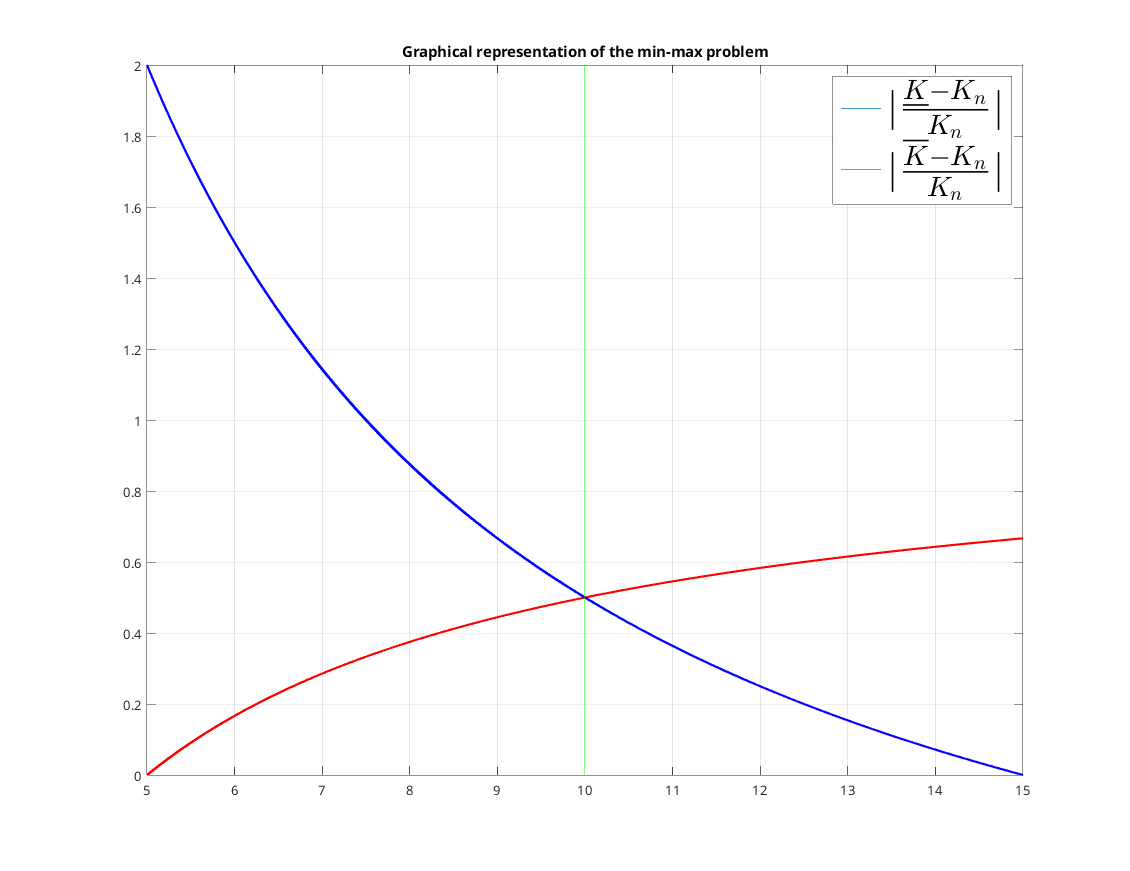
\includegraphics[width=0.5\textwidth]{minmax.png}
    \caption{Graphical representation of the minimization problem.}
\end{figure}

\begin{QandAbox}[Convervativeness Issue of unstructured uncertainty model sets]
Here, we remark that unstructured uncertainty model sets can only provide consvervative description of parametric uncertainties since, as shown in the previous exmaple, a complex function $\Delta(s)$ is used to account for the source of uncertainty, which is a real number. The unstructured uncertainty model set describes at each ferquency $\omega$ the uncertainty as a disk of radius $|W_u(j\omega)L_n(j\omega)|$ which is a conservative description of the actual uncertainty as shown in the following figure.
\end{QandAbox}
\begin{QandAbox}
\begin{figure}[H]
    \centering
    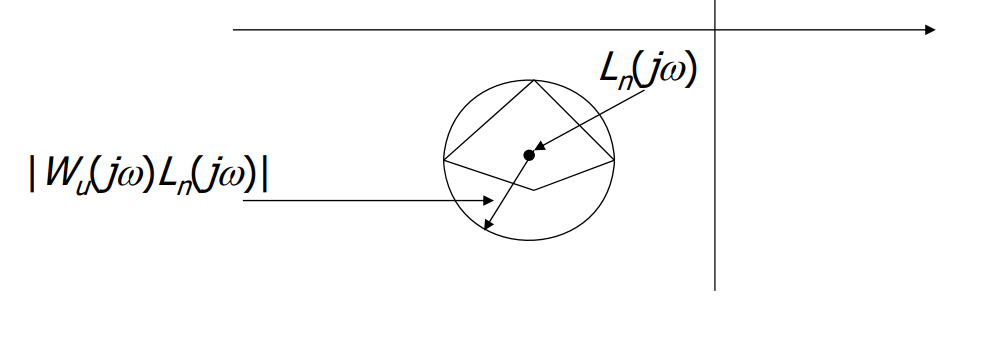
\includegraphics[width=0.75\textwidth]{conservative.png}
    \caption{Graphical representation of the conservetiveness issue of unstructured uncertainty model set.}
\end{figure}
\end{QandAbox}

\subsection{The inverse additive uncertainty model set}
The mathematical set of this kind of uncertainty model is as follows:
\[
M_m = \{G_p(s):\:G_p(s)\,=\,\frac{G_{pn}}{[1 + W_u(s)\Delta(s)G_{pn}(s)|},\,\|\Delta(s)\|_\infty\leq 1 \}
\]
\begin{figure}[H]
    \centering
    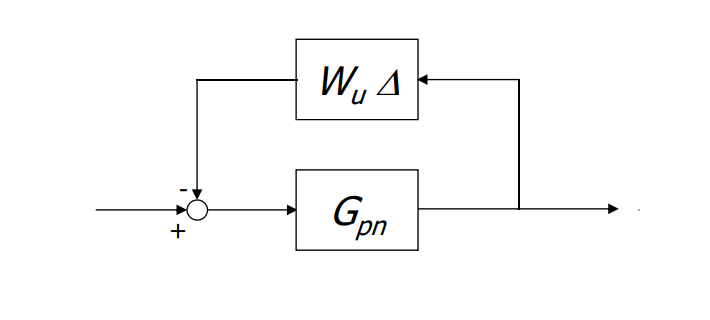
\includegraphics[width=0.5\textwidth]{inverse-additive.png}
    \caption{The block diagram description of inverse additive uncertainty}
\end{figure}

\subsubsection{Use cases:}
\begin{enumerate}
    \item \textbf{Uncertainty in System Poles:}\\
    \textbf{Scenario:} When the primary source of uncertainty affects the system’s poles rather than its zeros.\\
    \textbf{Why Inverse Additive:} Inverse additive uncertainty is effective in capturing changes in the denominator of the transfer function, which correspond to variations in the system poles.\\
    \textbf{Example:} A suspension system in a vehicle where damping ratios and natural frequencies are uncertain due to wear and environmental conditions.

    \item \textbf{Robustness to Controller Parameter Mismatch:}\\
    \textbf{Scenario:} When discrepancies between the designed and implemented controller parameters affect closed-loop behavior.\\
    \textbf{Why Inverse Additive:} Controller mismatch typically introduces pole shifts, which are well-represented by perturbations in the denominator.\\
    \textbf{Example:} A PID controller implemented with slightly incorrect gains, causing minor shifts in the closed-loop poles.

    \item \textbf{Dominance of Denominator Variations at Low Frequencies:}\\
    \textbf{Scenario:} When uncertainties in the system predominantly affect the low-frequency response due to variations in the denominator.\\
    \textbf{Why Inverse Additive:} At low frequencies, changes in the denominator significantly influence system behavior, making inverse additive uncertainty suitable.\\
    \textbf{Example:} A power grid experiencing load variations that alter the low-frequency impedance characteristics.

    \item \textbf{System Parameter Drift Over Time:}\\
    \textbf{Scenario:} When system parameters, such as time constants or damping ratios, drift over time due to aging or operational conditions.\\
    \textbf{Why Inverse Additive:} Parameter drifts primarily affect the poles of the transfer function, which are effectively modeled using inverse additive uncertainty.\\
    \textbf{Example:} An aging mechanical system where spring stiffness or damping properties degrade over time.

    \item \textbf{Uncertain Pole Placement in Control Design:}\\
    \textbf{Scenario:} When designing controllers for pole placement and the exact pole locations of the system are uncertain.\\
    \textbf{Why Inverse Additive:} This type of uncertainty directly represents variations in the desired pole locations.\\
    \textbf{Example:} A spacecraft attitude control system where uncertain moments of inertia introduce variability in the poles of the closed-loop transfer function.
\end{enumerate}



\subsection{The inverse multiplicative uncertainty model set}
The mathematical set of this kind of uncertainty model is as follows:
\[
M_m = \{G_p(s):\:G_p(s)\,=\,\frac{G_{pn}}{[1 + W_u(s)\Delta(s)|},\,\|\Delta(s)\|_\infty\leq 1 \}
\]
\begin{figure}[H]
    \centering
    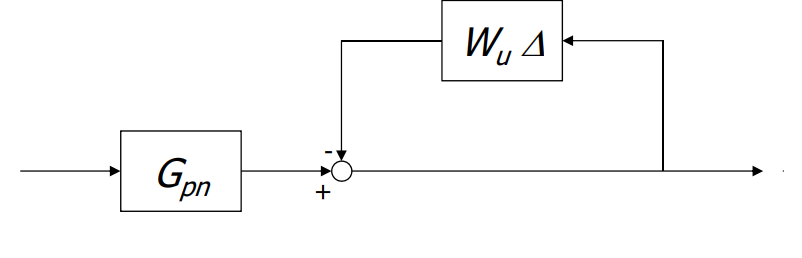
\includegraphics[width=0.5\textwidth]{inverse-multiplicative.png}
    \caption{The block diagram description of inverse additive uncertainty}
\end{figure}

\subsubsection{Use cases:}
\begin{enumerate}
    \item \textbf{Uncertainty in System Zeros:}\\
    \textbf{Scenario:} When the primary source of uncertainty affects the system’s zeros rather than its poles.\\
    \textbf{Why Inverse Multiplicative:} Inverse multiplicative uncertainty captures variations in the numerator of the transfer function, corresponding to changes in the system zeros.\\
    \textbf{Example:} An audio equalizer with varying zero locations due to inaccuracies in filter design.

    \item \textbf{Frequency-Dependent Uncertainty:}\\
    \textbf{Scenario:} When uncertainty is frequency-dependent and affects the system gain significantly at certain frequencies.\\
    \textbf{Why Inverse Multiplicative:} Frequency-dependent uncertainties are well-represented by scaling terms in the inverse multiplicative form.\\
    \textbf{Example:} A radio frequency amplifier with varying gain due to component aging or manufacturing tolerances.

    \item \textbf{Variations in System Gain:}\\
    \textbf{Scenario:} When uncertainties primarily influence the system gain, causing variations in the overall magnitude response.\\
    \textbf{Why Inverse Multiplicative:} Gain variations directly affect the numerator of the transfer function, aligning with the inverse multiplicative structure.\\
    \textbf{Example:} A hydraulic actuator where supply pressure fluctuations cause variability in the system's output gain.

    \item \textbf{Modeling Errors in High-Frequency Dynamics:}\\
    \textbf{Scenario:} When high-frequency dynamics introduce errors in the numerator of the transfer function.\\
    \textbf{Why Inverse Multiplicative:} Errors in high-frequency dynamics are often well-approximated by perturbations in the numerator, especially in systems where poles remain stable.\\
    \textbf{Example:} An industrial motor drive system with unmodeled high-frequency electrical effects.

    \item \textbf{System Behavior under Uncertain Input Conditions:}\\
    \textbf{Scenario:} When the system’s response is sensitive to input variations or disturbances, introducing uncertainty in the output.\\
    \textbf{Why Inverse Multiplicative:} The sensitivity of the system to input variations can often be modeled as changes in the numerator dynamics.\\
    \textbf{Example:} A robotic manipulator where input torque uncertainties affect the system’s trajectory.
\end{enumerate}

\textbf{From now on, we consider only multiplicative uncertainties for our systems.}

In order to chose the weight function, a practical way is to plot different members of the family, 10 sample at least for each parameter, and then consider $W_u$ to be a transfer function passing the maximum of all the magnitudes, shown in the following figure.
\begin{figure}[H]
    \centering
    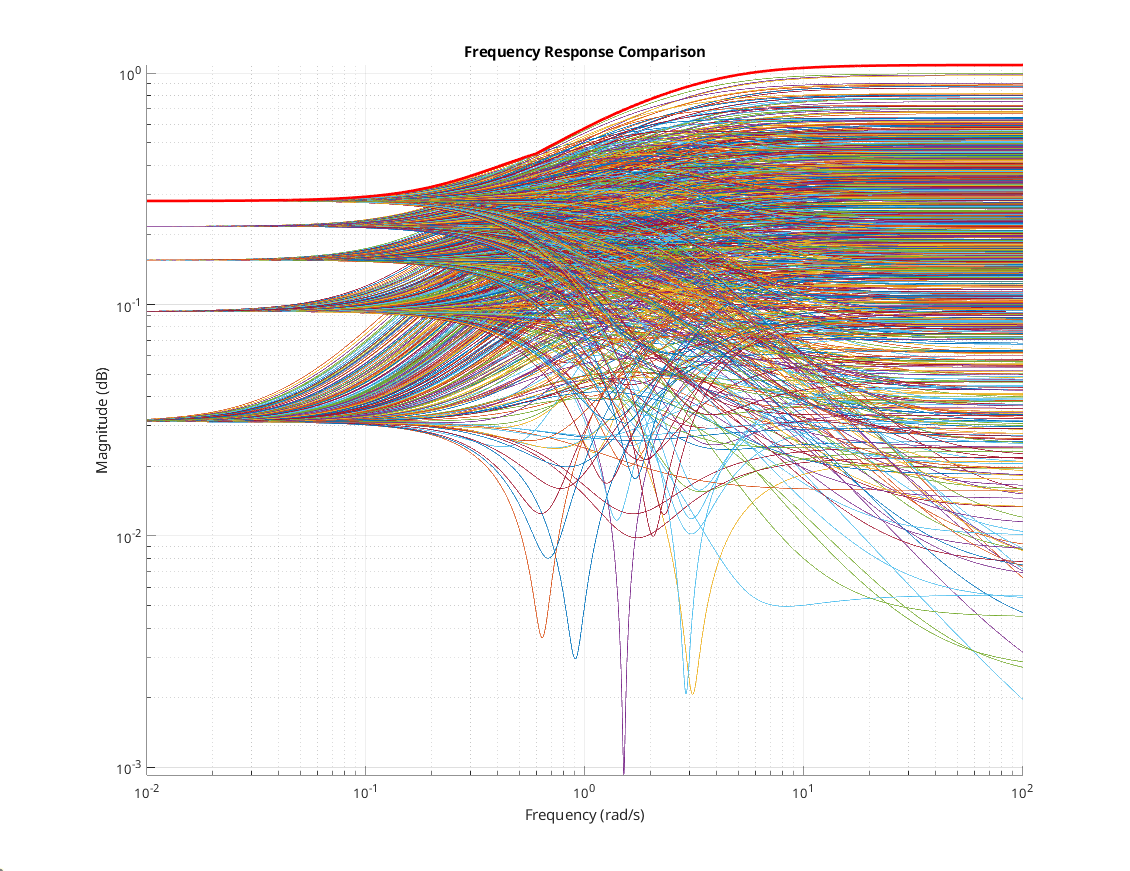
\includegraphics[width=1\textwidth]{uncertainty-weighting.png}
    \caption{The bold red plot is the transfer function that satisfies the inequality considered for $\delta$}
\end{figure}
FOR THE CODE, CHECK LABORATORY 06

The fitting tool, 'magfit()' command in matlab, used for finding $W_u$, usually returns a strictly proper transfer function, while it is recommended to model the uncertainty as fit as possible to the maximum value of the data, so in some cases, we may need to remove one or two zeros at this end. In the following figure, the blue dashed line is the output of the fitting tool, and the black dashed line is the modified weighting function.

\begin{figure}[H]
    \centering
    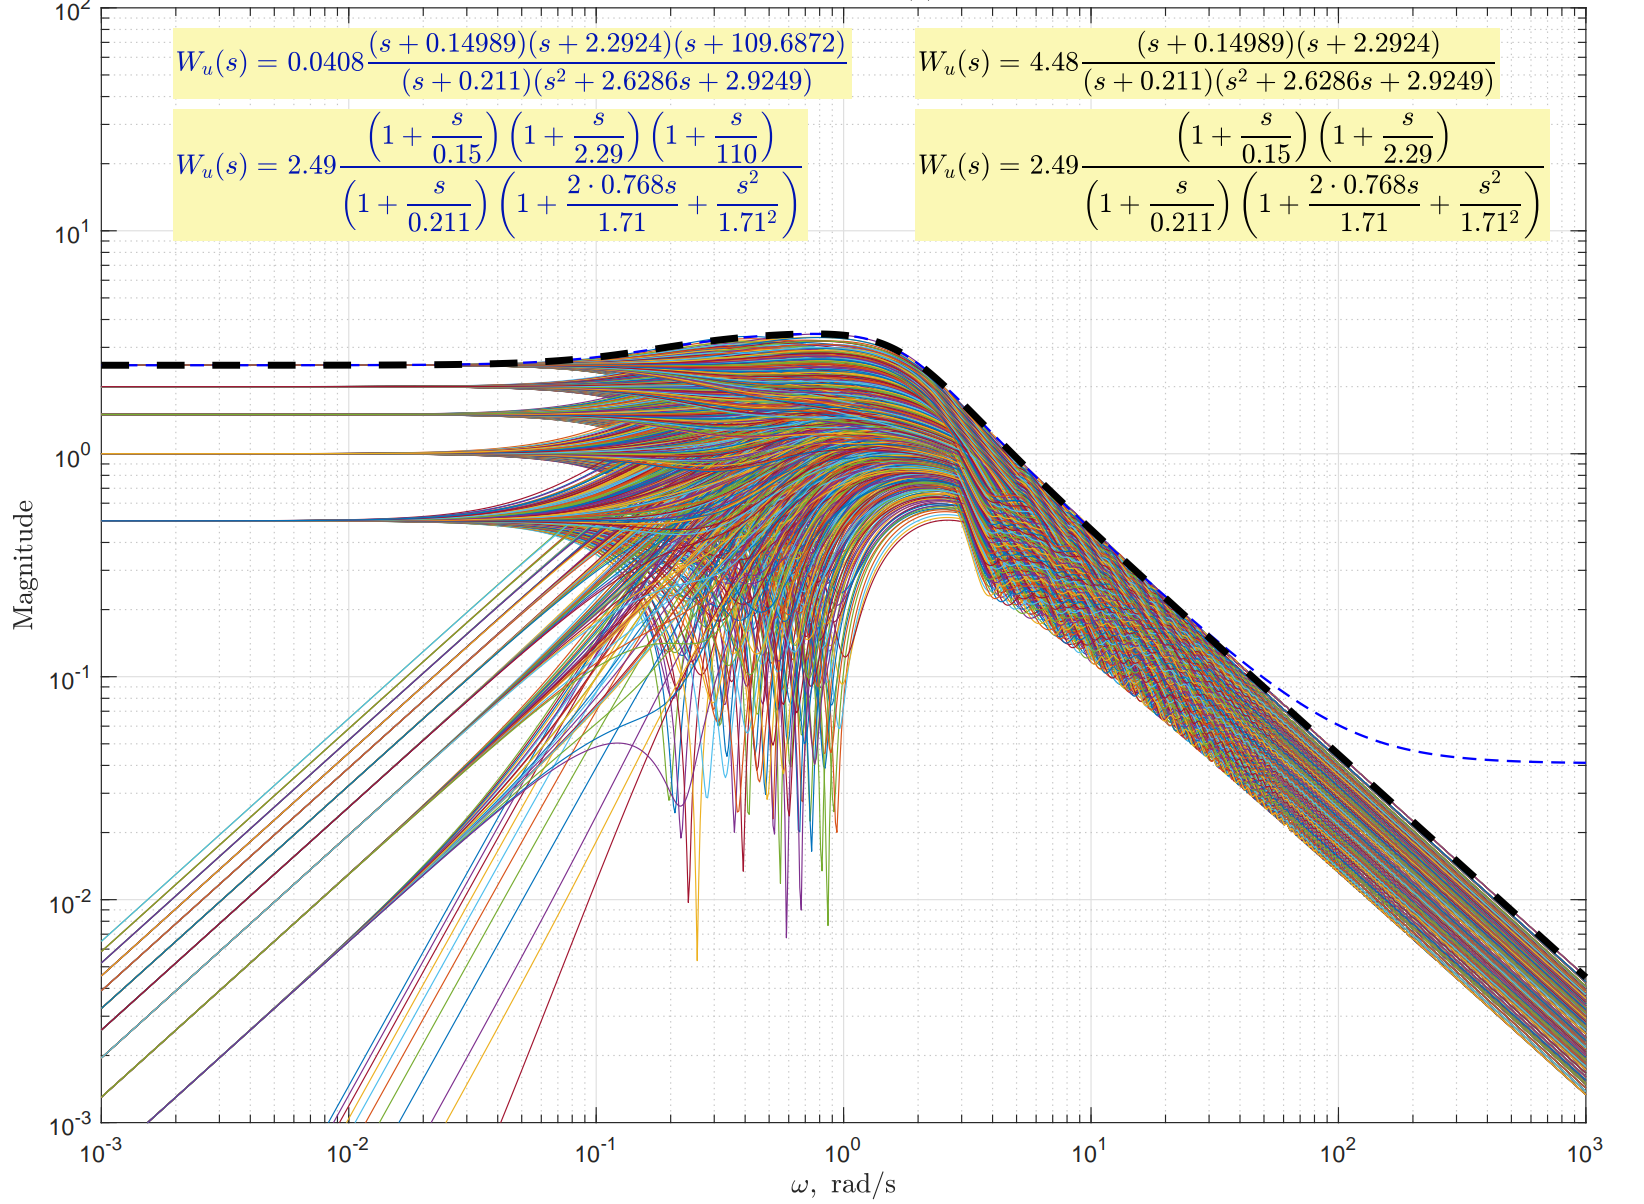
\includegraphics[width=1\textwidth]{Wu-proper.png}
    \caption{The plot of the uncertainties for the models of the model set and the corresponding strictly proper and proper $W_u$.}
\end{figure}

\begin{factbox}
In the low frequency range and middle frequency range, we should have $W_u$ pretty tight, but it can be loose in the high frequency range, because $T$ is a low pass transfer function and at high frequnecies its value is low. Nonetheless, it is recommended to make $W_u$ everywhere as tight as possible.\\
Another note that try to make the degree of the weighting function as low as possible. By doing so, the degree of the resultant controller is going to be low as well.
\end{factbox}

\begin{QandAbox}
In $\mu$ analysis, we can use linear algebra tools to obtain an upper and lower bounds for parameter uncertainties. As a result, for a given performance, how precise should the description of the plant be.
\end{QandAbox}
\section{Robust stability}
We aim at studying the stability of this feedback control system under the assumption that $G_p$ is an uncertain system describe by a given uncertainty model set. In particular, as it was mentioned, we assume, here, that $G_p$ belogns to a multiplicative uncertainty model set $M_m$.

\subsubsection{Definition (Robust Stability)}
The feedback system in the figure is \textbf{robustly stable} if and only if it is internally stable for each $G_p$ which belongs to $M_m$.
\[
M_m = \{G_p(s): G_p(s) = G_{pn}[1+W_u(s)\Delta(s)],\|\Delta(s)\|_\infty \leq 1\}
\]
\begin{figure}[H]
    \centering
    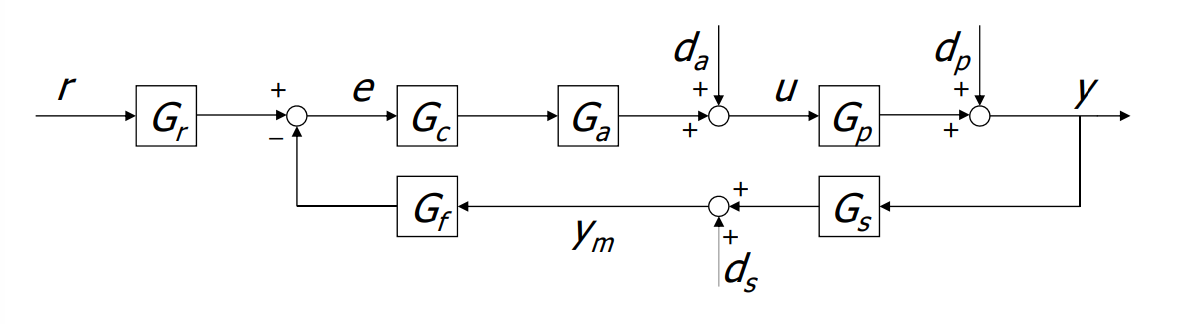
\includegraphics[width=1\textwidth]{block-scheme.png}
    \caption{The block diagram scheme of the feedback control system.}
\end{figure}

\subsubsection{Result (Robust Stability and multiplicative uncertainty)}
Assume that $G_p$ belogns to $M_m$, and assume that the feedback control system is stable when the nominal model $G_{pn}$ is considered as the model of the plant. The feedback system is \textbf{robustly stable} if and only if the following condition is satisfied:
\[
\|W_uT_n\|_\infty < 1
\]

where $Tn$ is the nominal complementary sensitivity function:d
\[
T_n = \frac{L_n}{1 + L_n}
\]
Where $L_n$ is the loop shaping function made by $G_{pn}$.


\subsection{sketch of the proof}
Let us define the nominal loop function as $L_n$. Since the feedback control system is stable for $G_p = G_{pn}$ by hypothesis, we know from the Nyquist criterion that the Nyquist plot of $L_n$ does not pass through the point -1 and its number of counter-clockwise encirclements equals the number of the poles of $L_n$ with positive real part.

As to the uncertain system, from the Nyquist theorem, we know that the feedback control system is robustly stable for $G_p = G_{pn}(1 + W_u\Delta)$ if and only if the Nyquist plot of $L = L_n(1 + W_u\Delta)$ does not cross the point $-1$ and its number of counter-clockwise encirlements equals the number of poles of $L_n$ with positive real part. we have that:
\[
L = L_n(1+W_u\Delta) \Rightarrow L-L_n = L_n W_u\Delta
\]
where
\[
\|\Delta(s)\|_\infty \leq 1 \Rightarrow |\Delta(j\omega)|\leq 1 \:\:\:\:\: \forall \omega
\]

\begin{figure}[H]
    \centering
    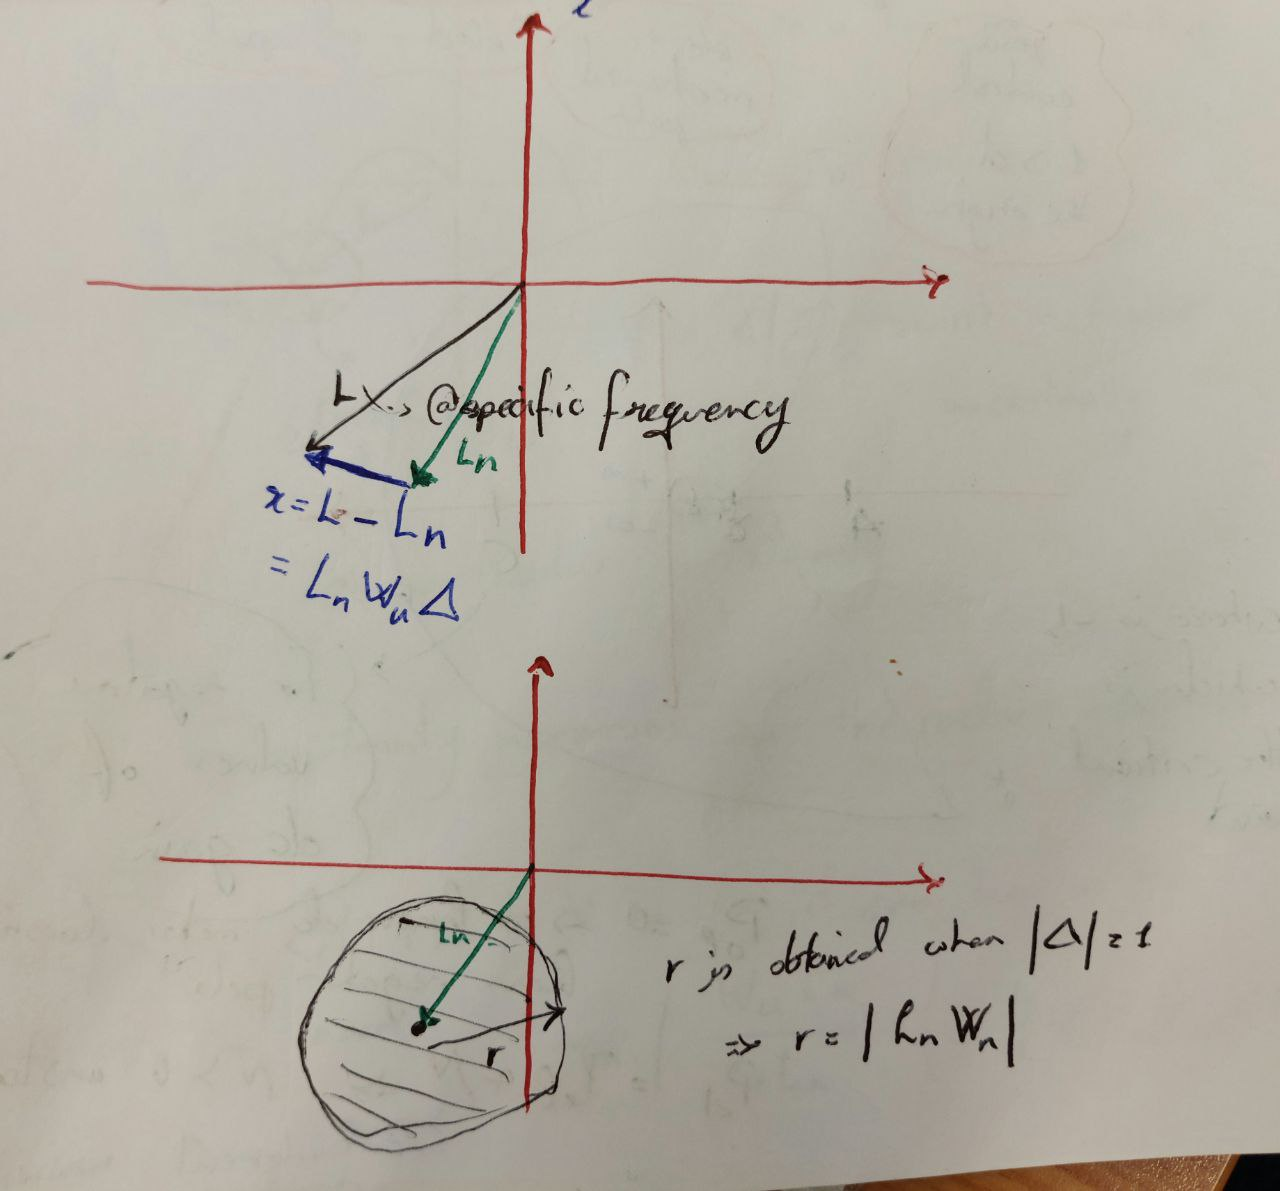
\includegraphics[width=0.6\textwidth]{L-Ln.jpg}
    \caption{Graphical representation of $L-L_n$ on the complex plane for a given frequency}
\end{figure}

\begin{figure}[H]
    \centering
    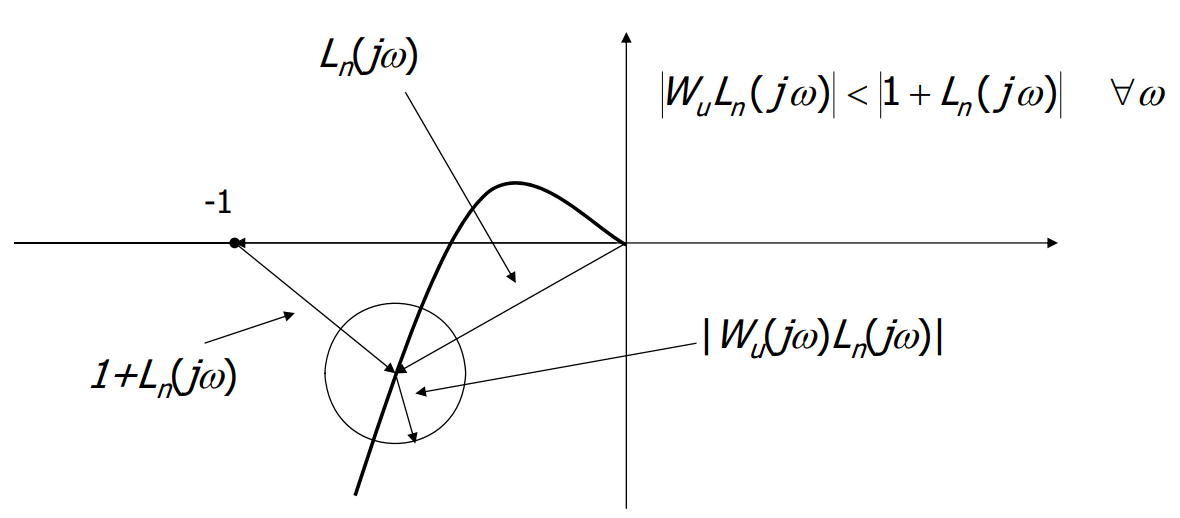
\includegraphics[width=0.75\textwidth]{robust-stability.png}
    \caption{The representation of the uncertainty disk.}
\end{figure}
It can be seen that if uncertainty increases, the circle approaches -1.
Since the uncertainty must not change the number of encirclements, the following condition for robust stability is obtained:
\[
|W_uL_n(j\omega)|\leq|1+L_n(j\omega)| \:\:\:\:\: \forall \omega
\]

which is equivalent to:
\[
\sup\limits_{\omega}|\frac{W_uL_n(j\omega)}{1+L_n(j\omega)}|=\|W_uT_n\|_\infty \leq 1
\]

\begin{example}[Example for Nyquist theorem]
Consider the transfer function of a feedback control system for position control of an electrical motor. The qualitative Nyquist plot of the loop function is shown in the following figure.
\begin{figure}[H]
    \centering
    \includegraphics[width=0.75\textwidth]{nyquist.jpg}
    \caption{Qualitative nyquist plot of an electric motor with position control.}
\end{figure}
Based on whether -1 is at the points A, B, or C, the stability characteristic of the nominal plant changes.\\
(A) $N = 0$, the nominal system is \textbf{stable}\\
(B) $N = 2$, the nominal system is \textbf{unstable} with two positive poles.\\
(C) $N = 1$ the system is unstable with one positive pole.
\end{example}
Robust statability condition for the remaining three uncertainty model sets can be obtained in a similar way. The following result summarizes the robust stability conditions for the four uncertainty model set considered. Note that $S_n = 1 - T_n$.
\begin{figure}[H]
    \centering
    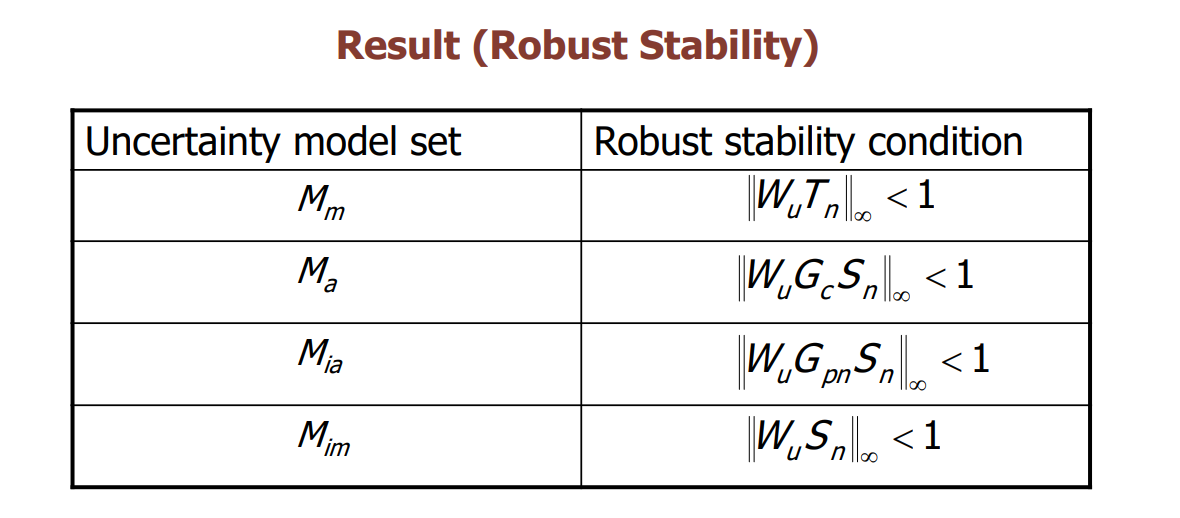
\includegraphics[width=0.75\textwidth]{robust-stability-results.png}
    \caption{The robust stability results for the four unstructured uncertainty models.}
    \end{figure}

\begin{QandAbox}[Very important point to be considered]
Pay attention that due to the conservativeness issue of unstructured uncertainty model sets. If the disk does not surpasses -1 for all the frequencies. We are sure that the system is robustly stable. However, \textbf{if for some frequencies the disk surpasses, it does not mean that the system is for sure robustly unstable.}\\

    Consider the following transfer function with the gain K being uncertain.
\[
G_{pn}(s) = \frac{K}{s(1+\frac{s}{p_1})(1+\frac{s}{p_2})}
\] 
In this case, the real uncertainty is on the length of L , while the multiplicative unstructured uncertainty introduces a disk at each frequency. which is not true. This disk may crosses -1 for some frequencies while the true system is robustly stable.

\begin{figure}[H]
    \centering
    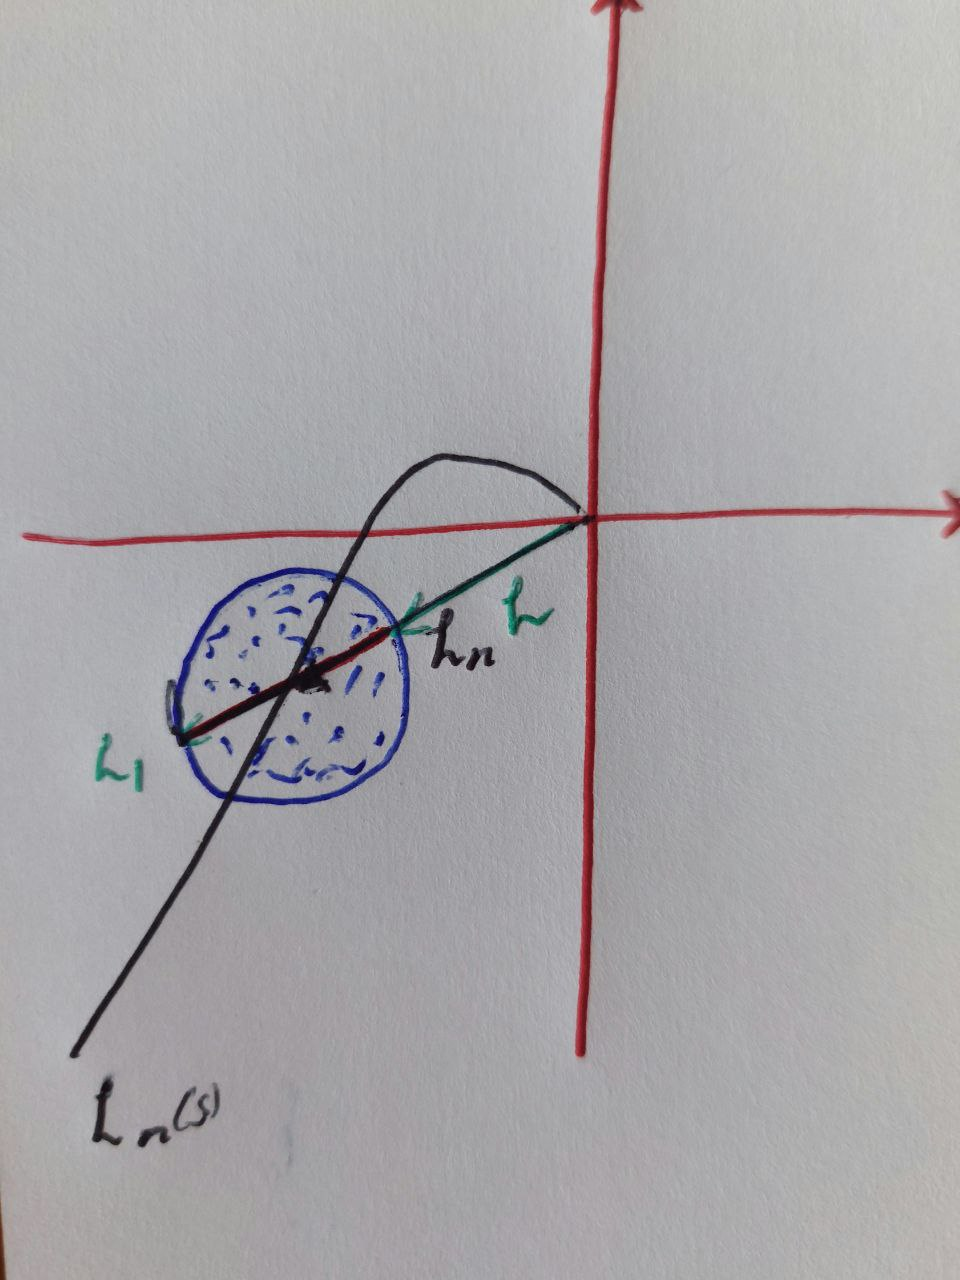
\includegraphics[width=0.5\textwidth]{true-uncertainty.jpg}
    \caption{The qualitative polar plot of the abovementioned transfer function.}
\end{figure}
   

\end{QandAbox}
\section{Nominal performance}
\begin{factbox}[professor's quote]
Always check the performance through time-domain simulation. The reason is that the translation of the requirements in frequency domain is not exact, we used the 2nd-order prototype system guidline, which does not tend to be the exact description of the system. \\
Another reason for checking the real-time performance is the conservativeness issue of unstructured uncertainty modelling.
\end{factbox}

\begin{QandAbox}[Performance limitatioons]
The crossover frequency should be larger that half of the real part of a system with non-minimum pole and should smaller than that for a system with a non-minimum zero. For further reading, take a look at the main source book pages 112 to 115.
\end{QandAbox}

Here, we recall the nominal performance conditions (i.e. performance conditions in the uncertainty-free case) derived previously. Performance requirements affecting the sensitivity function leads to the following condition;
\[
\|W_SS_n\|_\infty \leq 1 \Leftrightarrow |1 + L_n(j\omega)| > |W_s(j\omega)| \forall \omega
\]
while performance requirements affecting the complementary sensitivity function are translated into:
\[
\|W_TT_n\|_\infty \leq 1 
\]

\begin{figure}[H]
    \centering
    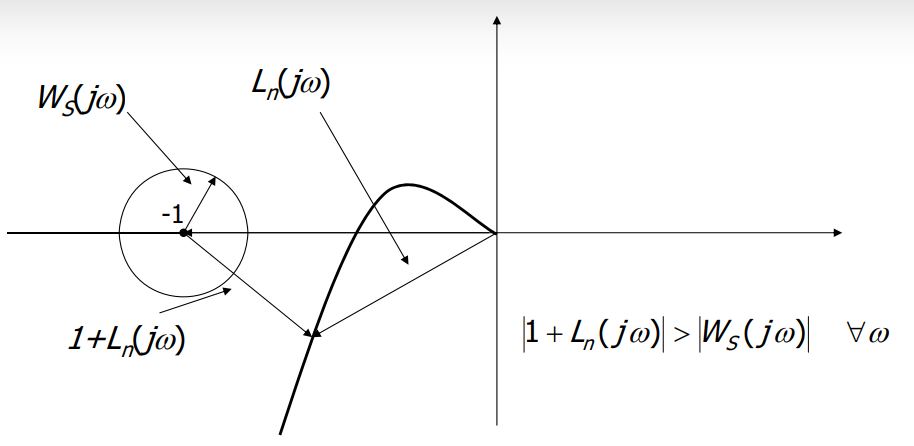
\includegraphics[width=0.75\textwidth]{nominal-performance.png}
    \caption{The qualitative polar plot showing nominal performance requirement on sensitivity.}
\end{figure}

Regarding the Bode plot, $W_S$ and $S_n$ must be exact when $s$ tends to zero and at the pick, while for the transient this is not the case.


\begin{figure}[H]
    \centering
    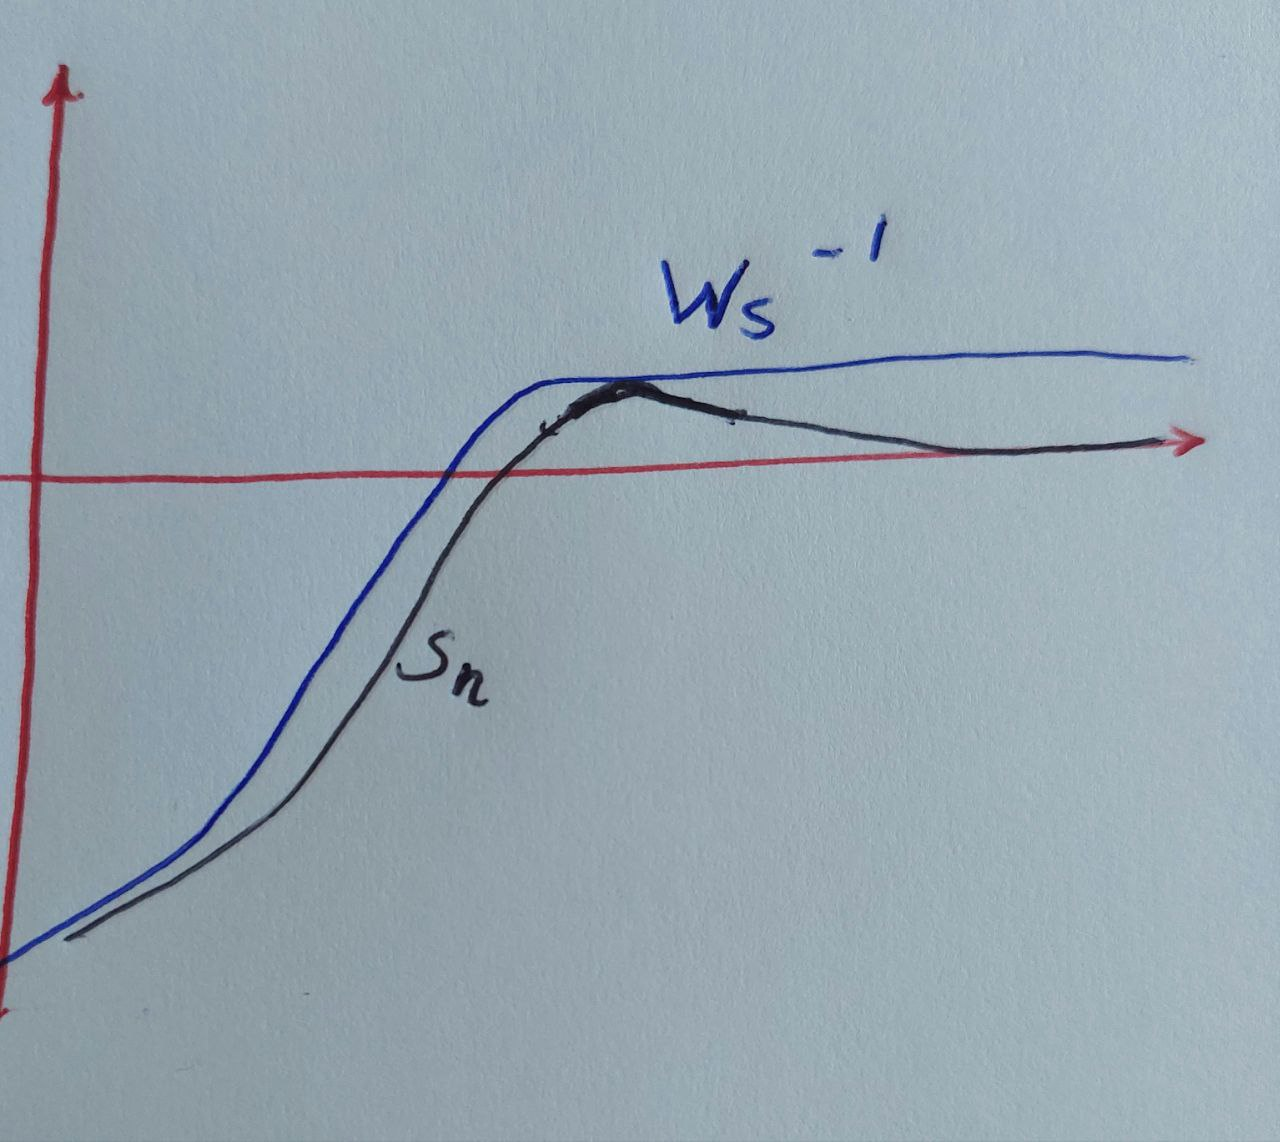
\includegraphics[width=0.5\textwidth]{nominal-performance-1.jpg}
    \caption{The nominal performance}
\end{figure}


\section{Robust performance}
\subsection{Definition}
The feedback system guarantees robust performance if and only if the performance requirements are satisfied for each $G_p$ which belongs to the given uncertainty model set.

Here, we consider the particular case where: 
\begin{itemize}
    \item performance requirements affect only the sensitivity function
    \item uncertainty is described by menas of a multiplicative model set $M_m$
\end{itemize}

The following result provides necessary and sufficient conditions for robust performance under such assumptions.

\subsection{Result}
The feedback system guarantees robust performance if and ony if the following condition is satisfied:
\[
\|W_SS_n||+|W_uT_n|\|_\infty < 1
\]
\subsection{Sketch of the proof}
By definition, the feedback system guarantees robust performance if and only if:
\[
\|W_SS\|_\infty < 1
\]
where
\[
S = \frac{1}{1+L_n(1+W_u\Delta)}
\]
thus, we can write the following robust performance condition:
\[
\|\frac{W_S}{1+L_n(1+W_u\Delta)}\|_\infty < 1
\]

which, being $L = L_n(1+W_u\Delta)$, can be equivalently written as:
\[
|1+L(j\omega)| > |W_S(k\omega)| \forall \omega
\]

This last condition means that at each frequency the loop function of th euncertaint system must stay outside the circle of radius $|W_S(j\omega)|$ centered at -1. \\
Now, let us consider the following relation straightforwardly derived from the definition of multiplicative uncertainty model set on the loop transfer function:
\[
|L(j\omega)-L_n/(j\omega)| \leq |W_u(j\omega)L_n(j\omega)| \:\:\:\:  \forall \omega
\]


From the following figure, it is clear that the feedback system guarantees robust performance if and only if the two disks do not overlap.


\begin{figure}[H]
    \centering
    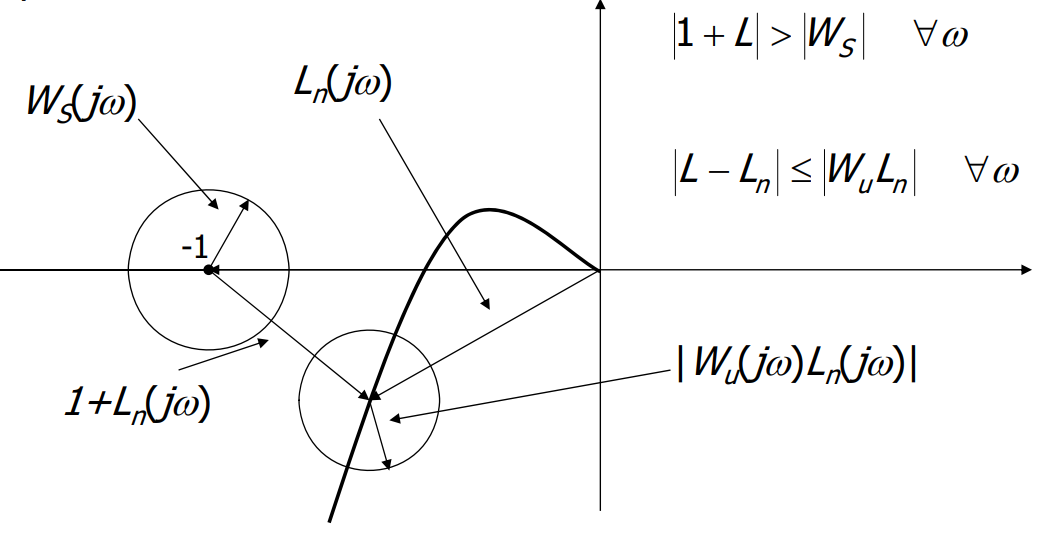
\includegraphics[width=0.5\textwidth]{robust-performance.png}
    \caption{The graphical reasoning for robust performance}
\end{figure}


The condition to avoid overlapping of of the two disks can be formally written as:
\[
\begin{array}{c}
|W_S|+|W_uL_n|<|1+L_n| \:\:\:\forall \omega \Leftrightarrow
|\frac{W_S}{1+L_n}|+|\frac{W_uL_n}{1+ L_n}|<1  \:\:\:\forall \omega
\\
\Leftrightarrow
\||W_SS_n|+|W_uT_n|\|_\infty <1
\end{array}
\]

which is the condition stated in the result.

\begin{QandAbox}[Some comments]
I) If $W_u$ in the case of unstructured uncertainty crosses $W_{Tn}$, we cannot conclude that robust stability is not satisfied \textbf{becaues of the conservativeness issue} which was discussed. However, if they don't cross, we can be sure that the system is robustly stable, putting for the same argument.\\

II) Since T is a low pass filter, the effect of high-frequency poles and zeros is going to be reduces. So it can be seen that even if we have high-frequency uncertainties  in $W_u$, at high frequencies, the multiplication of $W_uT_n$ is going to be small.
\end{QandAbox}

\begin{factbox}[Curiosity]
?? In $\mu$-analysis, we may be able to use linear algebra tools to obtain upper-bounds and lower-bounds for the parameter uncertainties in order to guarantee certain performance requirements. ?? If this is the case, we can use it to design the identification problem much easier.
\end{factbox}












 \chapter{$H_\infty$ design for robust control}

\section{Robust control via classical loop-shaping}
First , we consider the problem of designing a robust controller $G_c$ by means of classical loop shaping techniques. To this aim we present a set of necessary and sufficient conditions for robust performance fulfillment in terms of the frequency response of the loop function $L(s)$. Some general guildlines are provided about the design of a controller $G_c$ which provides the desired shape of the loop function. Our attention is restricted to the case of $W_T = 0$.\\


The following result provides \textbf{necessary conditions} for \textbf{robust performance} fulfillment in terms of the frequency response of the loop function $L(s)$.\\

\subsection{Result (Necessary conditiono for the case $|W_u|< 1$)}

Assume that $|W_u| < 1$. If the feedback system is such that 
\[
\||W_sS_n|+|W_uT_n|\|_\infty < 1
\]
Then, the loop function satisfies the following constraints:
\[
|L(j\omega)| > \frac{|W_s(j\omega)|-1}{1 - |W_u(j\omega)|} \:\:\forall \:\: \omega
\]

\textbf{Remark:} $|W_u| < 1$ is usually satisfied only at low frequencies.\\

\subsection{Result (Necessary conditiono for the case $|W_S|< 1$)}
Assume that $|W_S|<1$. If the feedback system is such that \\
\[
\||W_SS_n|+|W_uT_n|\|_\infty < 1
\]
then the loop function satisfied the following constraints
\[
|L(j\omega)| < \frac{1-|W_s(j\omega)|}{|W_u(j\omega)|-1} \:\:\forall \:\: \omega
\]
\textbf{Remark:} $|W_S| < 1$ is usually satisfied only at high frequencies.\\

he following result provides \textbf{sufficient conditions} for \textbf{robust performance} fulfillment in terms of the frequency response of the loop function $L(s)$.\\


\subsection{Result (Suffiecient conditiono for the case $|W_u|< 1$)}

Assume that $|W_u| < 1$. If the loop function satisfied the following constraints
\[
|L(j\omega)|> \frac{|W_S(j\omega)|+1}{1-|W_u(j\omega)|} \:\:\: \forall \:\:\: \omega
\]
then the feedback system is such that 
\[
\||W_SS_n|+|W_uT_n|\|_\infty < 1
\]

\textbf{Remark:} Again $|W_u| < 1$ is usually satisfied only at low frequencies.\\


\subsection{Result (Sufficient conditiono for the case $|W_S|< 1$)}
Assume that $|W_S|<1$. If the feedback system is such that \\
then the loop function satisfied the following constraints
\[
|L(j\omega)| < \frac{1-|W_s(j\omega)|}{|W_u(j\omega)|-1} \:\:\forall \:\: \omega
\]
then the feedback system is such that 
\[
\||W_SS_n|+|W_uT_n|\|_\infty < 1
\]

\textbf{Remark:} Also in this case, $|W_S| < 1$ is usually satisfied only at high frequencies.\\

\subsection{conclusion}
Since typical shapes of $W_S$ and $W_u$ are such that:
\[
|W_S(j\omega)| \gg 1  \text{  at low frequency}
\]
\[
|W_u(j\omega)| \gg 1  \text{  at high frequency}
\]

the following 
\[
|L(j\omega)| > \frac{W_S(j\omega)}{1- |W_u(j\omega)|}
\]
is a \textbf{necessary and sufficient condition at low frequency}, and

the following 
\[
|L(j\omega)| < \frac{1- W_S(j\omega)}{|W_u(j\omega)|}
\]
is a \textbf{necessary and sufficient condition at high frequency}.

 \begin{figure}[H]
    \centering
    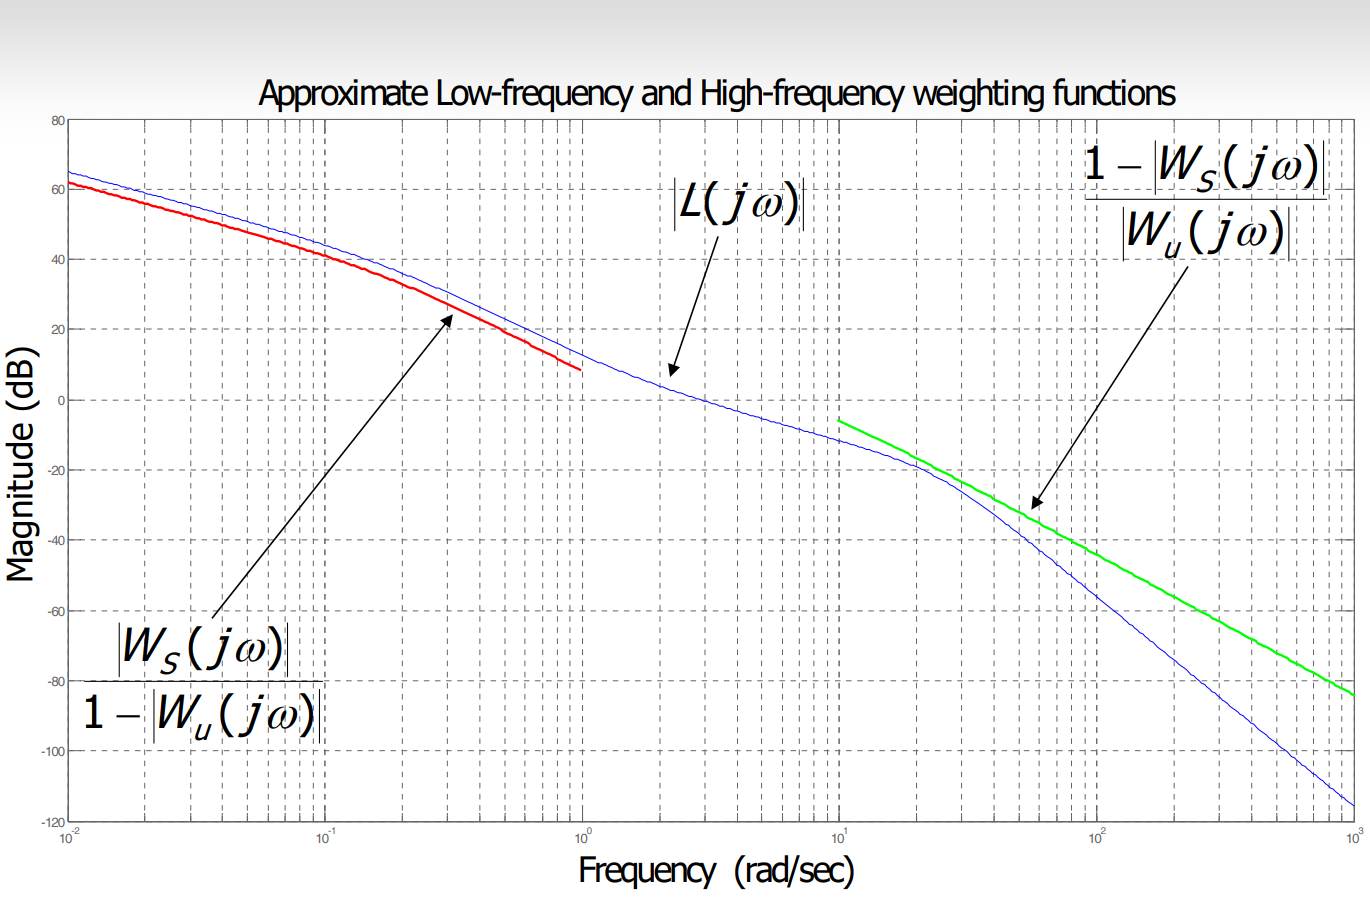
\includegraphics[width=0.75\textwidth]{robust-loop-shaping.png}
    \caption{Robust performance condition in the context of classical loop shaping.}
 \end{figure}

The obtained necessary and sufficient conditions provide traints on the magnitude of  the loop function at low and high frequencies.\\

As to the frequency range in the neighborhood of $\omega_c$, the loop function must be shaped in such a way to guarantee good stability.\\

\subsection{Controller design guidelines}
\begin{itemize}
    \item Select $\omega_c$ on the basis of the transient response requirements and the high and the low frequency range constraints on the magnitude of $L$.
    \item Select the gain $K_c$ and the number of poles of $G_c$ at $s=0$ in such a way as to satisfy the low frequency range constraints on the magnitude of $L$.
    \item Add the required lead/lag networks to satisfy the constraints related to the desired value sof $T_p$ and $S_p$ (the Nichols chart might help).
\end{itemize}

\section{Robust control via $H_\infty$ norm minimization}


First of all, let us recall the definition of he $H_\infty$ norm of a SISO LTI system with transfer function $H(s)$:
\[
\|H(s)\|_\infty = \max\limits_{\omega} |H(j\omega)|
\]
While the definition of the $H_\infty$ norm of a MIMO LTI system with transfer function $G(s)$ is:
\[
\|G(s)\|_\infty = \max\limits_{\omega} \bar{\sigma}(G(j\omega))
\]
where $\bar{\sigma}$ is the maximum singular value of $G(j\omega)$ for all $\omega$
This is the definition of the generalized norm. In the MATLAB, the command \texttt{norm(G,inf)} should be used.

\textbf{A different approach is presented now, where the controller $G_c$ is obtained by solving a suitable optimization problem.}\\

We consider general control problem where:
\begin{itemize}
    \item The plant is described by means of one of the four unstructured uncertainty model sets (additive, multiplicative, inverse additive, inverse multiplicative)
    \item  The norm performance requirements lead to the following conditions
    \[
    \|W_SS_n\|_\infty < 1 \hspace{1cm} \|W_TT_n\|_\infty<1
    \]
\end{itemize}

The $H_\infty$ norm minimization approach, called $H_\infty$ control, refers to a general formulation of the control problem which is based on the following block diagram representation of a general feedback system.

 \begin{figure}[H]
    \centering
    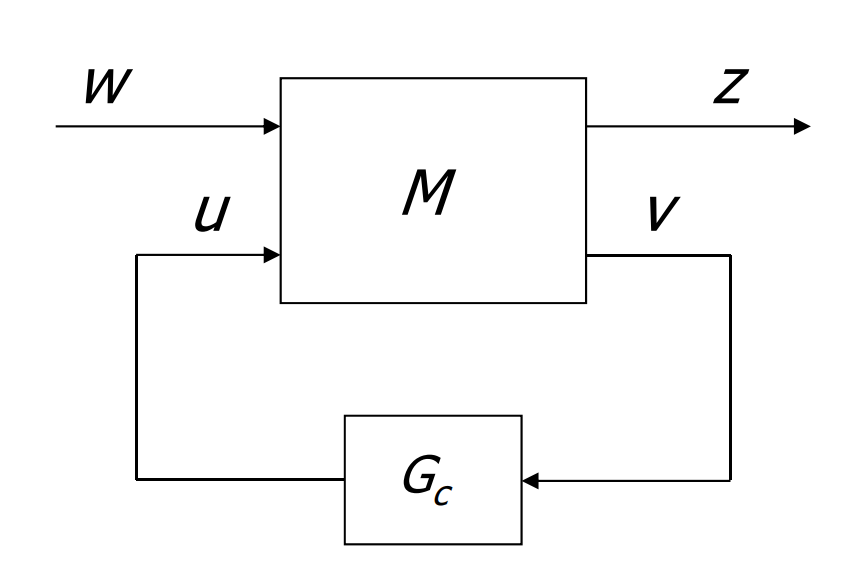
\includegraphics[width=0.5\textwidth]{gc-generalized-plant.png}
    \caption{The generalized plant considered for the control problem in the $H_\infty$ context.}
 \end{figure}
 
Where $M$ is the \textbf{generalized plant}, $G_c$ is the controller, $u$ is the vector of control inputs, $v$ is the vector of controller inputs, $w$ is the vector of external inputs, $z$ is the vector of external outputs, which can be used for the minimization of desirable criteria. \\

The external input and output signals of the generalized plant are not necessarily physical variables of the control system. The external input and output signals of the generalized plant must be carefully selected in order to take into account the stability/performance requirements of the considered control problem.\\

In the $H_\infty$ design, the controller is obtained by solving the following optimization problem
\[
G_c(s) = \arg \min\limits_{G_c \in G_c^{stab}} \|T_{wz}(s)\|_\infty
\]
$G_c^{stab}$ is the class of all the controllers which provide internal stability of the nominal feedback system.\\

$T_{wz}$ is the closed loop transfer function between the input $w$ and the output $z$

As previously stated, in $H_\infty$ control the controller $G_c$ is designed by minimizing the $H_\infty$ norm of the function $T_{wz}$.\\

Therefore, the key step is the proper selection of the generalized plant $M$ which must be build taking into account all the requirements of the considered control problem.\\

The design of the controller is performed in three steps:
\begin{itemize}
    \item select the transfer function $T_{wz}$
    \item build the generalized plant $M$ conrresponding the selected transfer function $T_{wz}$, which is the transfer function from the input $w$ to the output $z$.
    \item compute $G_c(s)$ by solving the optimization problem
    \[
    G_c(s) = \arg \min\limits_{G_c \in G_c^{stab}} \|T_{wz}(s)\|_\infty
    \]
    where as it was explained, $G_c^{stab}$ is the set of all the controllers which provide internal stability of the nominal feedback system.
\end{itemize}

If we find a controller $G_c$ that minimezes $W_uT_n$ and the result becomes less than 1 for all the frequencies, then the resultant controller is going to guarantee robust stability. Now, the question is that how to select $T_{wz}$?
\section{Generalized Plant for Robust Stability}
Now, let us consider the problem of designing a controller $G_c$ to robustly stabilize an uncertain system described by the unstructured multiplicative model set:
\[
M_m = \left\{G_p(s) = G_{pn}(s)[1 + W_u(s)\Delta(s)],\,\|\Delta(s)\|_\infty \leq 1\right\}.
\]
The condition for robust stability is known to be:
\[
\|W_uT_n\|_\infty < 1.
\]
In this case, we design a controller $G_c$ to minimize the weighted $H_\infty$ norm of a single transfer function. If the achieved minimum is less than 1, then the obtained controller robustly stabilizes the uncertain system.

The condition for robust stability is:
\[
\|W_uT_n\|_\infty < 1.
\]
The problem of designing a controller $G_c$ to satisfy the robust stability condition for unstructured multiplicative uncertainty can be solved by choosing the following transfer function $T_{wz}$:
\[
T_{wz}(s) = W_2T_n,
\]
where:
\[
W_2(s) = W_u(s).
\]
Assume, without loss of generality, that $G_f = G_s = G_a = 1$. The generalized plant $M$ corresponding to the selected transfer function $T_{wz}$ is the following (the portion inside the dashed box).

\begin{figure}[H]
    \centering
    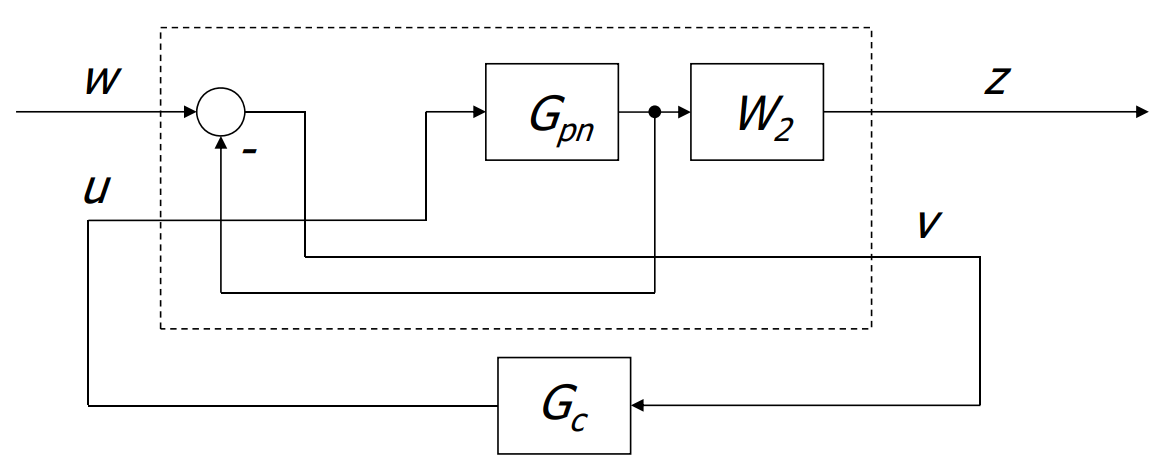
\includegraphics[width=0.75\textwidth]{gc-generalized-plant-robust-stability.png}
    \caption{The generalized plant considering the structure of our problem in the $H_\infty$ context.}
\end{figure}

\section{Generalized Plant for Nominal Performance}
Now, let us consider the problem of designing a controller $G_c$ to satisfy nominal performance:
\[
\|W_SS_n\|_\infty < 1, \hspace{0.5cm} \|W_TT_n\|_\infty < 1.
\]
\textbf{In this case, the goal is to design a controller $G_c$ that minimizes both of these weighted $H_\infty$ norms.} If the achieved minimum is less than 1, then the obtained controller satisfies the assigned nominal performance requirements.

To achieve this objective, we exploit the following result on the $H_\infty$ norm of a stack of transfer functions:

\subsection{Result (Norm of a Stack of Transfer Functions)}
\[
\left\|
\begin{array}{c}
H_1 \\
H_2 \\
\vdots \\
H_i \\
\vdots \\
H_n
\end{array}
\right\|_\infty
< 1
\implies
\|H_i\|_\infty < 1, \quad \forall i.
\]
According to this result, the minimization of the $H_\infty$ norm of $n$ transfer functions can be performed by minimizing the $H_\infty$ norm of the stack of such transfer functions ("stacking procedure").

\subsection{Result (Conservativeness of the Stacking Procedure)}
\[
\|H_i\|_\infty = 1 \quad \forall i \implies 
\left\|
\begin{array}{c}
H_1 \\
H_2 \\
\vdots \\
H_i \\
\vdots \\
H_n
\end{array}
\right\|_\infty
= \sqrt{n}.
\]
This result shows that the $H_\infty$ norm of a stack of transfer functions is (in the worst case) $\sqrt{n}$ times the value of the $H_\infty$ norm of each single transfer function.

Thus, the problem of designing a controller $G_c$ to satisfy the following nominal performance conditions:
\[
\|W_SS_n\|_\infty < 1, \hspace{0.5cm} \|W_TT_n\|_\infty < 1,
\]
can be solved by choosing the following transfer function $T_{wz}$:
\[
T_{wz} =
\begin{bmatrix}
W_1S_n \\
W_2T_n
\end{bmatrix},
\]
where:
\[
W_1(s) = W_S(s), \quad W_2(s) = W_T(s).
\]

\begin{figure}[H]
    \centering
    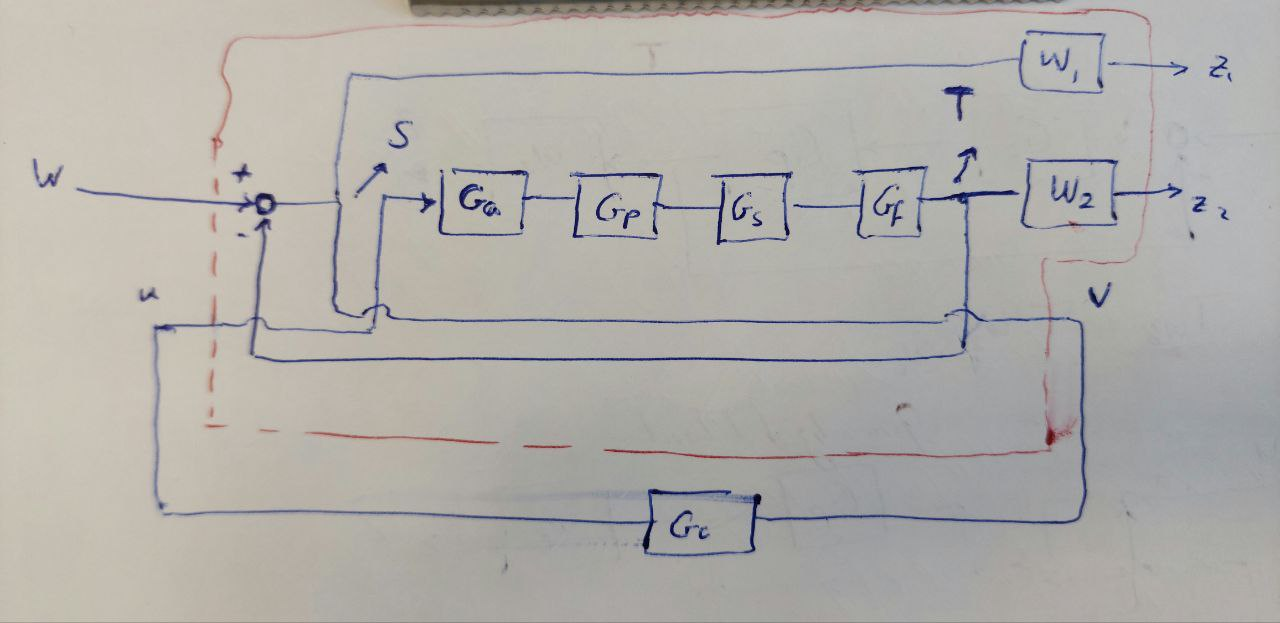
\includegraphics[width=0.5\textwidth]{gc-generalized-plant-2.jpg}
    \caption{The generalized plant considering the structure of our problem in the $H_\infty$ context.}
\end{figure}

\section{Generalized Plant for Nominal Performance (NP) and Robust Stability (RS)}
Finally, let us consider the problem of designing a controller $G_c$ to satisfy \textbf{both} nominal performance and robust stability conditions. In this case, the controller $G_c$ must be such that:
\[
\|W_SS_n\|_\infty < 1, \hspace{0.5cm} \|W_TT_n\|_\infty < 1, \hspace{0.5cm} \|W_uT_n\|_\infty < 1.
\]

The complementary sensitivity function must satisfy the following frequency domain constraints:
\[
|T_n(j\omega)|\leq|W_T^{-1}(j\omega)|,\quad |T_n(j\omega)|\leq|W_u^{-1}(j\omega)|, \quad \forall \omega.
\]

Thus, the problem of designing a controller $G_c$ which robustly stabilizes the given uncertain system and fulfills the nominal performance requirements can be solved by choosing the following transfer function $T_{wz}$:
\[
T_{wz} =
\begin{bmatrix}
W_1S_n \\
W_2T_n
\end{bmatrix},
\]
where \( W_1(s) = W_S(s) \) and \( W_2(s) \) is such that for each \(\omega\):
\[
|W_2(j\omega)| = \max(|W_u(j\omega)|,\,|W_T(j\omega)|).
\]

\begin{figure}[H]
    \centering
    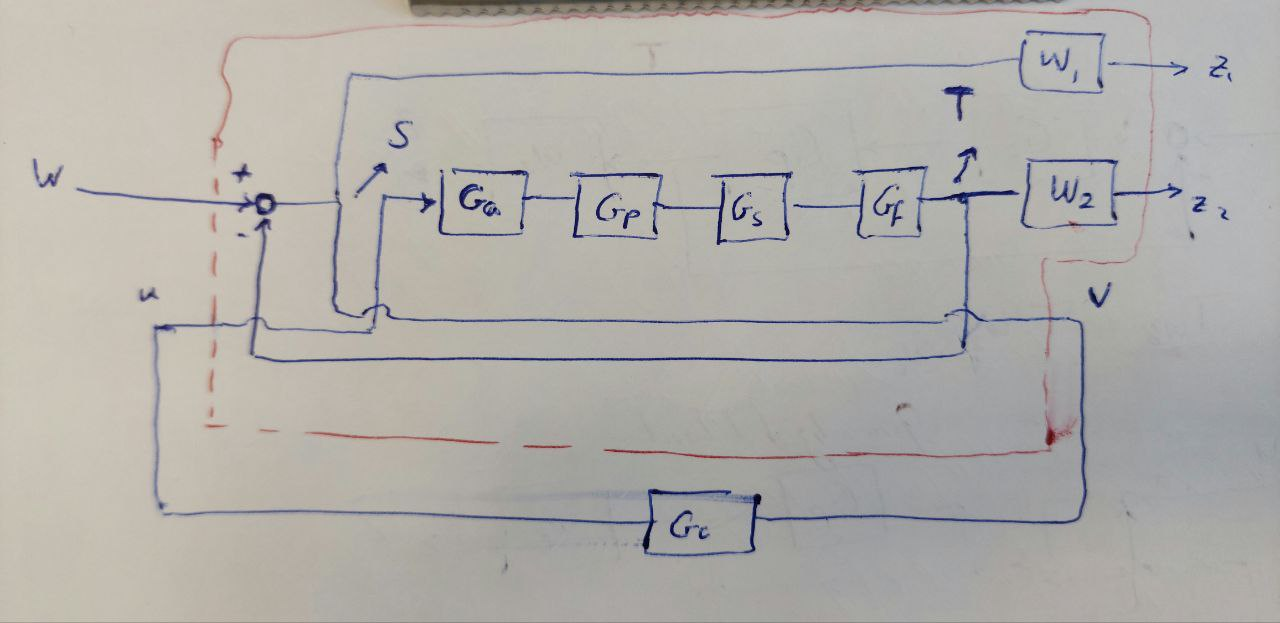
\includegraphics[width=0.5\textwidth]{gc-generalized-plant-2.jpg}
    \caption{The generalized plant considering the structure of our problem in the $H_\infty$ context.}
\end{figure}

Control problems involving constraints on the $H_\infty$ norm for more than one closed-loop transfer function are called \textbf{mixed sensitivity problems}. Examples include:
\begin{itemize}
    \item Designing $G_c$ to fulfill nominal performance requirements, leading to $H_\infty$ norm constraints on both $S_n$ and $T_n$.
    \item Designing $G_c$ to fulfill both nominal performance and robust stability requirements. (For this problem look at the last chapter of the book Doyle).
\end{itemize}

The controller design problem obtained by applying the \textbf{stacking procedure} to a mixed sensitivity problem is referred to as a \textbf{stacked mixed sensitivity problem}.

 \section{$H_\infty$ control: LMI optimizatino approach}
 As previously stated in the $H_\infty$ control, the controller is designed by solving the following optimization problem:
 
 \[
 G_c(s) = \arg \min\limits_{G_c \in G_c^{stab}} \|T_{wz}(s)\|_\infty
 \]
 
 Among the approaches proposed in the literature which solve such an optimization problem, we exploit the one based on the solution of a suitable constrainted optimization problem where the constraints are in the form of \textbf{Linear Matrix Ineqaulities} (LMI).\\
 
 The LMI based approach is implemented in the MATLAB LMI constrol system toolbox.\\
 
The LMI approach is based on a state-space description of the generalized plant $M$, which is depicted in the following figure:
The scheme of the generalized plant is as follows:
\begin{figure}[H]
    \centering
    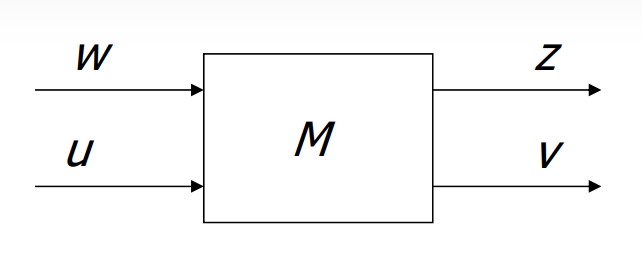
\includegraphics[width=0.5\textwidth]{generalized-plant.png}
    \caption{The scheme of the generalized plant.}
\end{figure}

\[
M: 
\begin{cases}
\dot{x}_M = A x_M + B_1 w + B_2 u\\
z = C_1 x_M + D_{11} w + D_{12} u\\
v = C_2 x_M + D_{21} w + D_{22} u
\end{cases}
\]

where \textbf{$x_M$ is the state vector of the generalized plant.} 

Referring to the mixed sensitivity problem, we have that:
\begin{itemize}
\item $x_M$ is given by the union of the state variables of the nominal model $G_{pn}$ and those of the weighting functions $W_1$ and $W_2$.
\item the eigenvalues of matrix $A$ are the union of the poles of the transfer functions $G_{pn}$, $W_1$, and $W_2$.
\end{itemize}

For the sake of simplicity and without loss of generality, assume that the controller $G_c$ to be designed is a SISO system (i.e. $u$ and $v$ are scalar signals).\\

The LMI optimization problem can be solved under the following mild assuptions:
\begin{itemize}
    \item[I] the matrix triplet ($A$,$B_2$,$C_2$) is stabilizable (i.e. if all unstable modes are controllable) and detectable (i.e. if all unstable modes are observable)
    \item[II] $D_{22} = 0$
\end{itemize}

Now, we will discuss the implementations of assumptions I and II on the solution of the mixed sensitivity problem. To this aim, let us consider again the generalizeed plant for the mixed sensitivity problem. 

\begin{figure}[H]
    \centering
    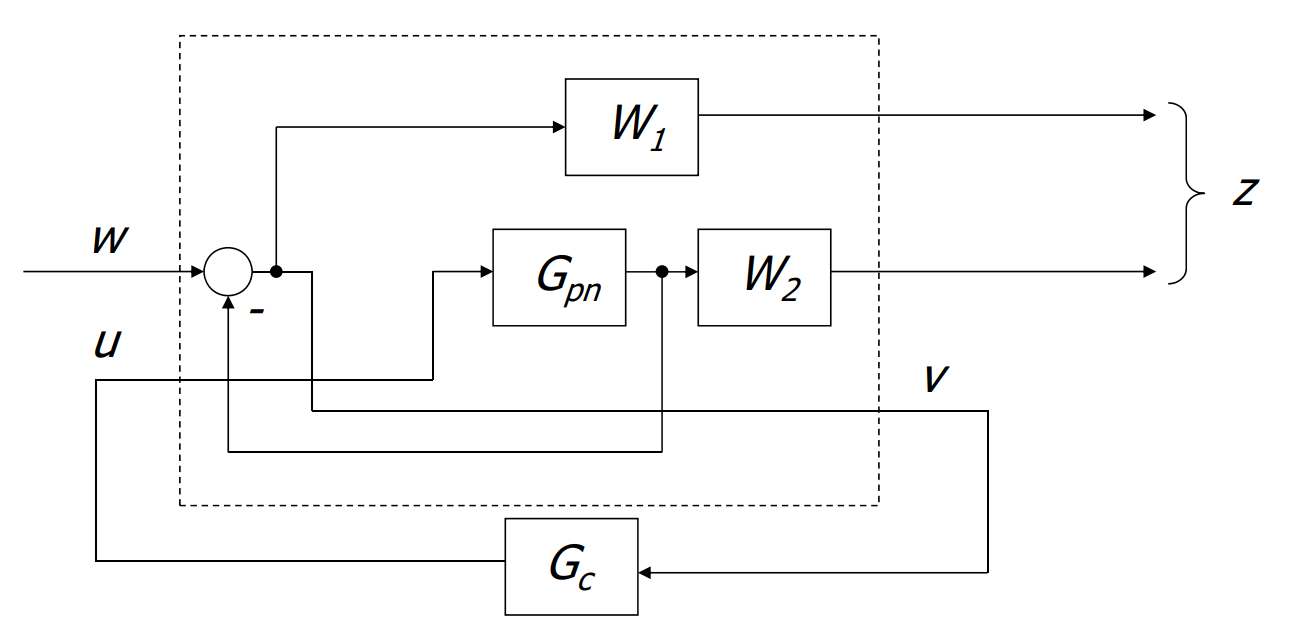
\includegraphics[width=0.75\textwidth]{mixed-sensitivity-problem.png}
    \caption{The scheme of the generalized plant for a mixed sensitivity problem}
\end{figure}

Consider the system described by the following equations (i.e. the generalized plant $M$ when only the input $u$ and the output $v$are considered)
\[
\begin{cases}
    \dot{x}_M = A x_M + B_2 u\\
z = C_1 x_M + D_{12} u\\
v = C_2 x_M + D_{22} u
\end{cases}
\]
Assumptions I requires that all the eigenvalues of the unobservable and uncontrollable part of this system are stable.\\

It easily seen from the block diagram of $M$ that all the modes of $A$ are controllable from $u$, while the modes of $A$ related poles of $W1$ and $W2$ are not observable from $v$.\\

Therefore, we have the following result:
\subsection{Result) Internal stability of the generalized plant $M$}
Consider the mixed sensitivity problem. The generalized plant 
$M$ can be internally stabilized by an LTI controller $G_c$ having input $v$ and input $v$ and output $u$ \textbf{if and only if} $W_1$ and $W_2$ are stable transfer functions.\\

Remark: This result requires that $W_1$ and $W_2$ are stable transfer functions. However, we know that some common performance requirements on the steady-state response to polynomial reference signals and disturbances lead to an unstable weighting function $W_1$ (due to the presence of one or more poles at $s = 0$)\\

Now, assume that the performance requirements are such that the weighting function $W_1$ has $\nu + p$ poles at $s = 0$.\\

In order to satisfy assumption I, we replace $W_1$ in the generalized plant $M$ with a new weighting function $W_1^{*}$ obtained as follows\\
\[
W_1^{*} = W_1 \frac{s^{\nu+p}}{(s + \lambda^{*})^{\nu + p}}
\]

So the modified $W_1$, $W_1^{*}$ is going to be as follows:

\begin{figure}[H]
    \centering
    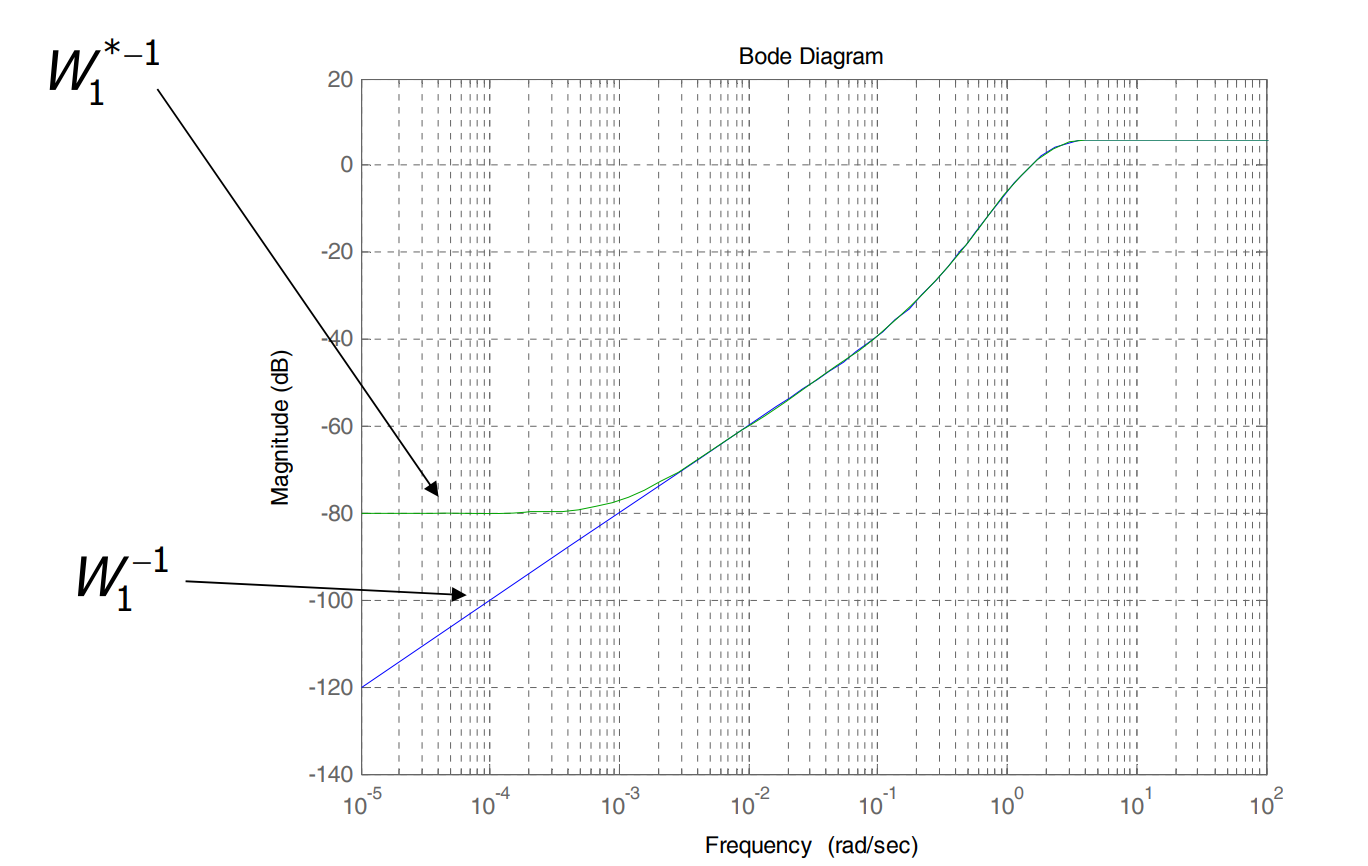
\includegraphics[width=0.75\textwidth]{modified-w1.png}
    \caption{The plot of the $W_1$ and its modified version,$W_1^{*}$}
\end{figure}


\begin{factbox}[About this kind of pole substitution]
Since the pole that is to be substituted has a frequency less than the cross over frequency of the weighting function, in this case a pole with frequency 0, in order no to modify the crossover frequency of the modified transfer function, the substitution should be sond in this zero-pole form $s + \lambda$, and not the dc-gain form. In this way, the dc-gain of the transfer function is adjusted such that the crossover frequency of the system does not change.\\

If the substitution or the cancellation is to be done on a pole or zero with a cutting frequency more than the crossover frequency, since the removal, or substitution does not affect the crossover frequency, there is no need so that the dcgain is modifies, so this operation can be done in the dcgain form ($1 + \frac{s}{\lambda^{*}}$), this is usefull for reducing the order of the controller obtained by the optimizer.
\end{factbox}

\newpage

\subsubsection{Need for modification of $W_2$}
$W_2$ is stable, but not proper, so we face a problem while creating the generalized plant in the Simulink, since it is not allowed to use uncausal blocks in Simulink. Hence, $W_2^{*}$ used in the Simulink block of the generalized plant $M$ is as follows:
\[
W_2^{*} = \frac{1}{T_{p0}}
\]
Now, in order to retreive the original form of $W_2$, in the command line the zeros are augmented,\\

\texttt{sderiv(M,2,[\textit{'the polynomial form of the derivator'}])} \\

where, 2 refers to the output channel on which the operation of derivative needs to be imposed, e.g. in the following $W_2$
\[
W_T = \frac{(1 + \frac{s}{p})(1 + \frac{s}{p})}{T_{p0}}
\]
\[
W_2^{*} = \frac{1}{T_{p0}}
\]
and in the command line, it need to be writen
\texttt{M = sderiv(M,2,[1/p 1])}
\texttt{M = sderiv(M,2,[1/p 1])}

\begin{factbox}[Experience]
According to the professor's experience, the optimizer return a better result for a generalized plant with real poles in the $W_2$. Therefore, another modification before doing the aforementioned modification is to make $W_2$ with real poles. 
\end{factbox}

\begin{QandAbox}[commands regarding $W_1^{*}$ and $W_2^{*}$]
Consider these two transfer functions as the nubs in order to obtain a better controller in terms of performance and simplicity. \\

For example, if the resultant loop function is not as fast as it is expected, by increasing the crossover frequency of $W_1$, one can force the optimizer to return a controller which results in a faster system, or if the overshoot need to be modified, the higher of $W_1$ or $W_2$ can be modified.
\end{QandAbox}

The following MATALB codes is to be used here:
\begin{itemize}
    \item \texttt{[Am, Bm, Cm, Dm] = linmod('simulink\_generalized\_plant')}\\
    \item \texttt{M = ltisys(Am, Bm, Cm, Dm)}\\
  
    \item If zeros need to be appended:\\
    \texttt{M = sderiv(M, 2, [1/p 1])}\\
    \texttt{M = sderiv(M, 2, [1/p 1])}\\
    
    \item \texttt{[g\_opt, Gc\_mod] = hinflmi(M, [1\ 1], 0, 0.01, [0\ 0\ 0])}\\
    \begin{itemize}
        \item \texttt{[1\ 1]} represents the number of inputs and outputs of the controller.
        \item \texttt{0} specifies gamma optimal (minimum achievable gamma).
        \item \texttt{0.01} defines the relative accuracy of the gamma optimum.
        \item \texttt{[0\ 0\ 0]} are optional parameters.
    \end{itemize}
    
    \item \texttt{[Ac, Bc, Cc, Dc] = ltiss(Gc_mod)}\\
    \item \texttt{Gc_mod = ss(Ac, Bc, Cc, Dc)}
\end{itemize}
Use minreal, to make sure cancellations are done.



% ---------------------------------------------------------------------
% ---------------------------------------------------------------------
% ---------------------------------------------------------------------

% Declare appendix and set the equation counter format to (A.section.eqNumber)
\appendix
\renewcommand{\theequation}{\thesection.\arabic{equation}}


\end{document}
